% =====================================================================
%  Abhijatri Project Proposal -- Team ChoturMatra
%  CSE 3102: Software Development Project
%  Compile with pdflatex (run twice for the table of contents).
%  Required file in the same folder: use-case-diagram.jpg
% =====================================================================
\documentclass[11pt,a4paper]{article}

% ---------- Fonts and encoding ----------
\usepackage[T1]{fontenc}
\usepackage[utf8]{inputenc}
\usepackage{mathptmx}                 % Times text and math
\usepackage[scaled=0.90]{helvet}      % Helvetica for sans-serif labels
\usepackage{microtype}

% ---------- Page layout ----------
\usepackage[a4paper,left=25mm,right=25mm,top=27mm,bottom=25mm,headheight=14pt,headsep=8mm]{geometry}
\usepackage{pdflscape}
\usepackage{fancyhdr}

% ---------- Tables, lists, figures ----------
\usepackage{graphicx}
\usepackage{booktabs}
\usepackage{longtable}
\usepackage{tabularx}
\usepackage{array}
\usepackage{multirow}
\usepackage{enumitem}
\usepackage{caption}
\usepackage{float}
\usepackage{needspace}
\usepackage{amsmath}
\usepackage{xcolor}
\usepackage{tikz}
\usepackage{afterpage}
\usepackage[section]{placeins}
\renewcommand{\topfraction}{0.9}
\renewcommand{\bottomfraction}{0.8}
\renewcommand{\textfraction}{0.08}
\renewcommand{\floatpagefraction}{0.85}
\setcounter{topnumber}{3}
\setcounter{totalnumber}{5}
\makeatletter
\setlength{\@fptop}{0pt}
\setlength{\@fpsep}{14pt plus 2pt}
\setlength{\@fpbot}{0pt plus 1fil}
\makeatother

% ---------- Headings and contents ----------
\usepackage{titlesec}
\usepackage{titletoc}
\usepackage[hidelinks]{hyperref}
\usepackage{url}

\hypersetup{
  pdftitle={Abhijatri Project Proposal},
  pdfauthor={Team ChoturMatra},
  pdfsubject={CSE 3102 Software Development Project},
  bookmarksnumbered=true,
  linktoc=all
}

% ---------- Paragraphs and lists ----------
\setlength{\parindent}{0pt}
\setlength{\parskip}{6pt plus 1pt}
\setlength{\emergencystretch}{2em}
\renewcommand{\arraystretch}{1.25}
\setlist[itemize]{label=\textbullet,leftmargin=1.6em,itemsep=3pt,topsep=4pt,parsep=0pt}
\setlist[enumerate]{label=\arabic*.,leftmargin=1.8em,itemsep=3pt,topsep=4pt,parsep=0pt}
\clubpenalty=10000
\widowpenalty=10000

% ---------- Section headings (research-paper style) ----------
\titleformat{\section}{\needspace{12\baselineskip}\large\bfseries}{\thesection}{0.8em}{}
\titleformat{\subsection}{\needspace{9\baselineskip}\normalsize\bfseries}{\thesubsection}{0.7em}{}
\titleformat{\subsubsection}{\needspace{4\baselineskip}\normalsize\bfseries}{\thesubsubsection}{0.6em}{}
\titlespacing*{\section}{0pt}{16pt}{6pt}
\titlespacing*{\subsection}{0pt}{12pt}{4pt}
\titlespacing*{\subsubsection}{0pt}{9pt}{3pt}

% ---------- Table of contents styling ----------
\setcounter{tocdepth}{2}
\contentsmargin{2.4em}
\dottedcontents{subsection}[4.3em]{}{2.6em}{0.6pc}
\titlecontents{section}[1.7em]{\addvspace{5pt}\bfseries}
  {\contentslabel{1.7em}}{\hspace*{-1.7em}}
  {\hfill\contentspage}
\titlecontents{figure}[2.6em]{\addvspace{3pt}}{\contentslabel{2.6em}}{}{\titlerule*[0.6pc]{.}\contentspage}
\titlecontents{table}[2.6em]{\addvspace{3pt}}{\contentslabel{2.6em}}{}{\titlerule*[0.6pc]{.}\contentspage}

% ---------- Captions: bold label, upright text ----------
\captionsetup{font=small,labelfont=bf,labelsep=period,justification=centering,skip=5pt}
\captionsetup[table]{position=top}
\captionsetup[longtable]{position=top}

% ---------- Header and footer ----------
\pagestyle{fancy}
\fancyhf{}
\fancyhead[L]{\small Abhijatri: Project Proposal}
\fancyhead[R]{\small Team ChoturMatra}
\fancyfoot[C]{\small \thepage}
\renewcommand{\headrulewidth}{0.4pt}
\renewcommand{\footrulewidth}{0pt}
\fancypagestyle{plain}{\fancyhf{}\fancyfoot[C]{\small\thepage}\renewcommand{\headrulewidth}{0pt}}

% ---------- Column types and helpers ----------
\newcolumntype{Y}{>{\raggedright\arraybackslash}X}
\newcolumntype{L}[1]{>{\raggedright\arraybackslash}p{#1}}
\newcolumntype{C}[1]{>{\centering\arraybackslash}p{#1}}
\newcolumntype{R}[1]{>{\raggedleft\arraybackslash}p{#1}}
\newcommand{\hd}[1]{\textbf{#1}}
\newcommand{\ganttfont}{\fontsize{7.2}{8}\selectfont}
\newcommand{\extlink}[2]{\href{#1}{\textbf{\underline{#2}}}}
\newcommand{\ganttsmall}{\fontsize{6.5}{7.2}\selectfont}

\begin{document}

% =====================================================================
%  TITLE PAGE
% =====================================================================
\begin{titlepage}
  \centering
  \vspace*{20mm}
  {\fontsize{30}{36}\selectfont\bfseries Abhijatri\par}
  \vspace{4mm}
  {\Large A Bangla-First, Offline-Ready Community Travel Platform for Bangladesh\par}
  \vspace{10mm}
  \rule{0.55\textwidth}{0.4pt}\par
  \vspace{6mm}
  {\large\bfseries Project Proposal\par}
  \vspace{2mm}
  {\large CSE 3102: Software Development Project\par}
  \vspace{16mm}

  \begin{tabular}{L{40mm}L{95mm}}
    \toprule
    \hd{Team}             & ChoturMatra \\
    \hd{Project type}     & Software development \\
    \hd{Platform}         & Bangla-first, offline-ready Progressive Web Application (PWA) \\
    \hd{Proposal date}    & 12 October 2026 \\
    \hd{Final completion} & 17 or 18 January 2027 \\
    \bottomrule
  \end{tabular}

  \vfill
  {\large\bfseries Team Members\par}
  \vspace{4mm}
  \begin{tabularx}{\textwidth}{L{36mm}L{48mm}Y}
    \toprule
    \hd{Responsibility} & \hd{Member} & \hd{Primary contribution} \\
    \midrule
    Project leader              & Shahriar Islam                & Scope control, content, estimator rules, administration, integration, and documentation \\
    Frontend and offline        & Abdullah Bin Sorwar Choudhury & React, TypeScript, bilingual interface, PWA, and offline packs \\
    Backend and data            & Syed Muhtasim Alam            & FastAPI, PostgreSQL, authentication, APIs, rating, and idempotency \\
    Software quality assurance  & Md.\ Irfan Iqbal              & Test strategy, validation, real-device testing, pilot, and regression \\
    \bottomrule
  \end{tabularx}
  \vspace{6mm}
\end{titlepage}

% =====================================================================
%  FRONT MATTER
% =====================================================================
\pagenumbering{roman}
\setcounter{page}{1}
\pdfbookmark[1]{Contents}{toc}
\tableofcontents
\clearpage
\pdfbookmark[1]{List of Figures and Tables}{lof}
\listoffigures
\vspace{8mm}
\listoftables
\clearpage
\pagenumbering{arabic}
\setcounter{page}{1}

% =====================================================================
\section*{Scope Decision}
\phantomsection
\addcontentsline{toc}{section}{\protect\numberline{}Scope Decision}
Abhijatri will be developed as a Bangla-first, offline-ready Progressive Web Application. The semester minimum viable product (MVP) is organized around one complete journey: a traveller explores a destination, generates a contextual cost estimate, downloads an offline travel pack, and submits a moderated review after reconnecting. Vendor commerce, real payments, group tours, and tourmate matching are future phases. A reservation and payment sandbox may be demonstrated only as a non-production extension; it is not part of semester acceptance.

% =====================================================================
\section{Executive Summary}
Travellers in Bangladesh often plan trips from social media posts, agency advertisements, personal blogs, maps, and informal recommendations. These sources vary in age, format, and reliability. They rarely explain why two trips to the same destination have different costs, and they become difficult to use when network access is weak.

Abhijatri is a community-driven travel platform designed for Bangladesh. It combines bilingual destination guidance, structured community reviews, transparent ratings, dated travel advisories, an explainable rule-based cost planner, and downloadable offline travel packs. Bangla is the default language; English is available through a persistent language control.

The semester outcome is a tested PWA with five seeded destination profiles: Cox's Bazar, Sajek, Sylhet, the Sundarbans, and Bandarban. The final demonstration will cover the destination, estimate, offline, review, and moderation flow. The platform will not use machine learning for cost prediction. It will use documented pricing rules, source dates, pricing units, season factors, low--expected--high ranges, and confidence labels.

% =====================================================================
\section{Problem Statement}
\subsection{Fragmented travel information}
Travel information for Bangladesh is distributed across many platforms. Users must compare content with different dates, assumptions, and commercial interests. Seasonal restrictions, permits, transport changes, verified contacts, and local guidance can be missed.

\subsection{Unclear trip costs}
A single average cannot represent a solo traveller, student, couple, family, or group. Accommodation can be priced per room, transport per person or per vehicle, meals per person, and guides per group or per day. A useful estimate must show the cost basis, the traveller context, and the source date.

\subsection{Weak connectivity}
Hill districts, rural areas, and remote destinations may have slow, unstable, or unavailable mobile data. Travellers can lose access to contacts, guidance, advisories, and cost details exactly when they need them. An online-only system does not meet this requirement.

\subsection{Limited Bangla-first support}
International travel services may provide reviews and maps, but they do not consistently provide Bangla-first guidance, Bangladesh-specific pricing units, local seasonality, and contextual cost explanations in one workflow.

\subsection{Trust, moderation, and freshness}
Community content can be duplicated, biased, or manipulated. Prices and travel restrictions also change. The system must show review counts, moderation status, source dates, confidence labels, and advisory validity. Expired information must not be presented as current.

% =====================================================================
\section{Objectives and Goals}
Each objective is measurable against the final completion date.

\begin{longtable}{L{10mm}L{46mm}L{88mm}}
\caption{Project objectives and completion measures}\label{tab:objectives}\\
\toprule
\hd{ID} & \hd{Objective} & \hd{Completion measure} \\
\midrule
\endfirsthead
\toprule
\hd{ID} & \hd{Objective} & \hd{Completion measure} \\
\midrule
\endhead
\bottomrule
\endlastfoot
O1 & Deliver a bilingual PWA & Bangla-default interface, persistent English selection, and installable application shell \\
O2 & Publish seeded destination profiles & Five profiles with bilingual guidance, dated sources, contacts, seasonality, and advisories \\
O3 & Provide explainable cost estimation & Itemized BDT estimate with pricing units, low--expected--high range, per-person cost, source dates, and confidence label \\
O4 & Provide dependable offline access & Every completed pack download opens successfully in 10 of 10 airplane-mode tests \\
O5 & Implement trustworthy reviews & Structured reviews, offline drafts, moderation states, reporting, and duplicate-safe submission \\
O6 & Evaluate estimator performance & Ten held-out trips evaluated after the seed catalogue is frozen, without tuning on those trips (Section~\ref{sec:planner-validation}) \\
O7 & Validate usability & At least eight consenting participants, including a Bangla-preferring user and a less technical user \\
O8 & Meet the reporting schedule & Biweekly evidence-based progress reports, formal testing from 4 to 11 January, and final completion on 17 or 18 January 2027 \\
\end{longtable}

% =====================================================================
\section{Functional Requirements}
\subsection{Core Product Features}
\begin{enumerate}
  \item \textbf{Bangla-first destination guides.} Users can explore destination profiles covering attractions, accommodation, food, transport, local practices, contacts, seasonality, and dated advisories in Bangla and English.
  \item \textbf{Structured community reviews.} Reviews include travel date, traveller type, comfort level, text, overall rating, and category ratings. Review counts and moderation status remain visible.
  \item \textbf{Transparent destination rating.} The platform uses a documented Bayesian score based on published overall ratings and a fixed semester prior. Hidden, rejected, and deleted reviews are excluded by tested query logic.
  \item \textbf{Context-based cost planner.} Users receive an itemized BDT estimate based on party size, traveller type, dates, duration, comfort tier, transport, accommodation, meals, and selected activities. The result separates shared and per-person costs (Section~\ref{sec:planner}).
  \item \textbf{Offline travel pack.} Users can download public destination guidance, contacts, coordinates, advisories, and the generated estimate. The pack remains available in airplane mode after a successful download.
  \item \textbf{Saved trip brief.} Users can save an estimate, free-text notes, and optional local contacts. This is a compact trip summary, not a day-by-day itinerary planner.
  \item \textbf{Offline review draft.} A review written without connectivity remains on the device and can be submitted after reconnection. Retry requests use an idempotency key to prevent duplicates.
  \item \textbf{Advisory freshness.} Every advisory stores its source, verification date, effective date, and validity date. Current, stale, and expired states are presented distinctly.
  \item \textbf{Lean moderation and administration.} Authorized users manage destinations, translations, prices, advisories, review decisions, reports, and audit records.
  \item \textbf{Privacy-aware account access.} Email verification controls review submission. The MVP does not collect real NID records, payment credentials, or unnecessary identity documents.
\end{enumerate}

\subsection{Future Product Features}
The following capabilities belong to the product vision but are not required for semester acceptance:
\begin{itemize}
  \item \textbf{Abhijatri Perks:} clearly disclosed partner benefits from approved resorts, restaurants, transport providers, and guides.
  \item \textbf{Vendor participation:} vendor registration, partner verification, reservation requests, ticket requests, and commission-based agency participation.
  \item \textbf{Find Tourmates:} verified organizers, join requests, capacity control, women-only options, participant visibility, private discussion, reporting, and blocking.
  \item \textbf{Advanced verification and payments:} real phone OTP, NID or student ID verification, verified-visit badges, real payments, refunds, and live inventory confirmation.
  \item \textbf{Platform expansion:} native mobile applications, advanced route planning, and context-aware machine learning once sufficient verified data exists.
\end{itemize}

\subsection{User Roles}
\begin{table}[H]
\centering
\caption{User roles and permitted actions}\label{tab:roles}
\begin{tabularx}{\textwidth}{L{40mm}Y}
\toprule
\hd{Role} & \hd{Permitted actions} \\
\midrule
Guest & Browse public destinations, switch language, generate estimates, and download public offline packs \\
Email-verified user & All guest actions plus saved trip briefs, review drafts, review submission, reporting, and account deletion request \\
Moderator & Review reports and publish, hide, reject, or flag content with a recorded reason \\
Administrator & Manage destinations, translations, prices, advisories, users, permissions, and audit records \\
\bottomrule
\end{tabularx}
\end{table}

\subsection{Functional Requirement Catalogue}
{\small
\begin{longtable}{L{11mm}L{28mm}L{43mm}L{59mm}}
\caption{Functional requirement catalogue}\label{tab:fr}\\
\toprule
\hd{ID} & \hd{Function} & \hd{Input} & \hd{Output or behaviour} \\
\midrule
\endfirsthead
\multicolumn{4}{l}{\small\textbf{Table \thetable} (continued)}\\
\toprule
\hd{ID} & \hd{Function} & \hd{Input} & \hd{Output or behaviour} \\
\midrule
\endhead
\bottomrule
\endlastfoot
FR01 & Destination catalogue & Destination selection & Bilingual profile with attractions, transport, food, lodging, contacts, dates, and restrictions \\
FR02 & Language selection & Bangla or English & Interface and available editorial content in the selected language \\
FR03 & Account lifecycle & Email, password, and verification link & Verified session, reset, logout, and deletion request \\
FR04 & Structured review & Rating, text, categories, and travel context & Pending review with a local draft retained until successful submission \\
FR05 & Review moderation & Review and moderation decision & Published, hidden, rejected, or deleted state with actor, date, and reason \\
FR06 & Review reporting & Published review and report reason & Moderator-visible report record with duplicate control \\
FR07 & Destination rating & Eligible published overall ratings & Fixed-prior Bayesian score and visible review count \\
FR08 & Cost planner & Party, traveller type, dates, comfort tier, transport, lodging, meals, and activities & Itemized BDT estimate with low, expected, and high values, per-person result, and confidence label \\
FR09 & Pricing units & Source-dated price records & Calculation by person, room, vehicle, group, trip, day, night, meal, or entry \\
FR10 & Offline pack & Destination and generated estimate & Versioned IndexedDB pack containing public guidance, contacts, coordinates, advisories, and costs \\
FR11 & Saved trip brief & Estimate, notes, and optional contacts & Local record with a UUID and copy or delete action \\
FR12 & Offline review draft & Review entered without connectivity & Local draft that survives refresh and session expiry \\
FR13 & Retry-safe submission & Review and idempotency key & One server review for identical retries \\
FR14 & Pack update & Existing pack and newer manifest & Atomic replacement after the new pack passes validation \\
FR15 & Advisory freshness & Source and validity dates & Current, stale, or expired state presented to the user \\
FR16 & Administration & Authorized management action & Updated public data and immutable audit event \\
FR17 & Storage control & Pack download or deletion request & Persistence status, storage notice, and local data removal \\
\end{longtable}
}

% ---------------------------------------------------------------------
\subsection{Abhijatri Cost Planner}\label{sec:planner}
\textbf{Purpose.} Travellers can find individual prices, but they rarely receive an estimate that explains how party size, travel dates, comfort tier, and shared costs change the total. The cost planner answers three practical questions before a trip: (i) can this group afford this trip, (ii) how should shared costs be divided fairly, and (iii) which choices (dates, comfort tier, transport) change the total most.

\textbf{Approach.} The MVP implements a deterministic rules engine. It does not use machine learning or probabilistic simulation, so every result can be reproduced by hand, reviewed, and tested. Each estimate is decision support, not a vendor quotation or a price guarantee.

\textbf{Terminology.} Two independent dimensions are used throughout. The \textbf{comfort tier} (economy, standard, or premium) is chosen by the user and selects which catalogue items apply. The \textbf{price range} (low, expected, or high) expresses the realistic spread of prices for the selected items within that tier.

\subsubsection{Inputs and outputs}
\begin{table}[!htbp]
\centering
\caption{Cost planner inputs and their effect on the calculation}\label{tab:planner-inputs}
{\small
\begin{tabularx}{\textwidth}{L{38mm}L{46mm}Y}
\toprule
\hd{Input} & \hd{Values} & \hd{Effect on the calculation} \\
\midrule
Destination and dates & Seeded destination; start and end date & Selects catalogue records and the season band of each chargeable day or night \\
Party & Party size $n$; traveller types (adult, student, child) & Sets the number of eligible travellers $n_e$ for person-based items and the capacity division for shared items \\
Duration & Days $d$ and nights $m$ & Sets the number of chargeable periods \\
Comfort tier & Economy, standard, or premium & Selects the accommodation, transport, and meal records that apply \\
Choices & Transport mode, accommodation type, meal plan, activities & Includes or excludes cost categories and items \\
\bottomrule
\end{tabularx}
}
\end{table}

For every category the result shows the low, expected, and high cost, the pricing unit, the quantity used, the source date, and the confidence value. It also shows the group total, the per-person share, the split between shared and individual costs, the assumptions applied, and an overall confidence label.

\subsubsection{Price catalogue}
Each price record stores the destination, category, item, comfort tier, season applicability, pricing unit, capacity, low price, expected price, high price, source type, source reference, verification date, validity date, and confidence. Records must satisfy $p^{L} \le p^{E} \le p^{H}$, and room, vehicle, and group records must state a capacity. Official sources take priority for fixed charges such as entry fees and permits. Recent moderated community reports are used for variable categories such as accommodation, food, and local transport.

\subsubsection{Deterministic calculation}
For each included category $i$ and each range value $v \in \{L, E, H\}$, the engine computes
\begin{equation}
K_i^{v} \;=\; p_i^{v} \times q_i \times \sum_{\tau \in T_i} s(\tau),
\label{eq:cost}
\end{equation}
where $p_i^{v}$ is the unit price for range value $v$, $q_i$ is the number of units required, $T_i$ is the set of chargeable periods, and $s(\tau)$ is the season factor of period $\tau$. The quantity and period rules are fixed per pricing unit (Table~\ref{tab:units}). Season factors are maintained in configuration for regular, weekend, peak, and public-holiday periods; fixed official charges always use $s(\tau) = 1$. Summing over periods, rather than applying one factor to the whole trip, correctly prices a trip that mixes weekday and weekend nights.

\begin{table}[!htbp]
\centering
\caption{Quantity and period rules by pricing unit}\label{tab:units}
{\small
\begin{tabularx}{\textwidth}{L{30mm}L{38mm}L{36mm}Y}
\toprule
\hd{Pricing unit} & \hd{Units required $q_i$} & \hd{Chargeable periods $T_i$} & \hd{Typical use} \\
\midrule
Per person       & $n_e$                    & One occurrence           & Intercity bus fare \\
Per entry        & $n_e$                    & One per visit            & Park or site entry fee \\
Per room         & $\lceil n / c_i \rceil$  & Each night ($m$)         & Hotel or resort room \\
Per vehicle      & $\lceil n / c_i \rceil$  & Each day used ($d$)      & Local jeep, CNG, or boat \\
Per group        & $\lceil n / c_i \rceil$  & Each day or one trip     & Guide or permit escort \\
Per meal         & $n_e$                    & Meals per day $\times\, d$ & Restaurant meals \\
Per day / night  & $1$                      & Each day or night        & Daily service charge \\
Per trip         & $1$                      & One occurrence           & Reserved transfer \\
\bottomrule
\end{tabularx}
}
\end{table}

Here $c_i$ is the capacity of one room, vehicle, or group unit, and $\lceil\cdot\rceil$ denotes ceiling division. The group totals and the per-person share are
\begin{equation}
T^{v} = \sum_i K_i^{v}, \qquad P^{v} = \frac{T^{v}}{n}.
\label{eq:total}
\end{equation}
Shared categories (rooms, vehicles, group services) are divided by party size only for the per-person view, and the result lists shared and individual amounts separately so the group can settle costs fairly. Calculations use unrounded values; displayed amounts are rounded to the nearest BDT 10.

\subsubsection{Worked example}
Table~\ref{tab:example} applies Equation~\eqref{eq:cost} to four students travelling to Cox's Bazar for three days and two nights (Thursday to Saturday) at the standard comfort tier. The first night is a regular night ($s = 1.00$); the second night and the last two days fall on the weekend ($s = 1.15$). \textbf{All prices in this example are illustrative placeholders used to demonstrate the rules; they are not researched catalogue values.}

\begin{table}[!htbp]
\centering
\caption{Worked example of the cost calculation (illustrative prices, BDT)}\label{tab:example}
{\small
\begin{tabularx}{\textwidth}{Y L{26mm} C{7mm} C{12mm} R{14mm} R{14mm} R{14mm} C{9mm}}
\toprule
\hd{Category} & \hd{Unit and rule} & \hd{$q_i$} & \hd{$\sum s(\tau)$} & \hd{Low} & \hd{Expected} & \hd{High} & \hd{$C_i$} \\
\midrule
Intercity bus (return) & Per person, fixed & 4 & 1.00 & 8,000 & 9,600 & 12,000 & 0.90 \\
Hotel room, capacity 2 & Per room, 2 nights & 2 & 2.15 & 9,460 & 12,900 & 17,200 & 0.70 \\
Meals, 3 per day & Per meal, 9 meals & 4 & 9.00 & 6,480 & 9,000 & 12,600 & 0.60 \\
Local vehicle, capacity 4 & Per vehicle, 3 days & 1 & 3.30 & 2,970 & 3,960 & 5,280 & 0.50 \\
Park entry (official) & Per entry, fixed & 4 & 1.00 & 200 & 200 & 200 & 0.95 \\
\midrule
\textbf{Group total $T^{v}$} & & & & \textbf{27,110} & \textbf{35,660} & \textbf{47,280} & \\
\textbf{Per person $P^{v}$} & & & & \textbf{6,780} & \textbf{8,920} & \textbf{11,820} & \\
\bottomrule
\end{tabularx}
}
\end{table}

Unit prices used (low / expected / high): bus 2,000 / 2,400 / 3,000 per person; room 2,200 / 3,000 / 4,000 per night; meal 180 / 250 / 350; vehicle 900 / 1,200 / 1,600 per day; entry 50. For example, the expected room cost is $3{,}000 \times \lceil 4/2 \rceil \times (1.00 + 1.15) = 12{,}900$. The shared share of the expected total (room and vehicle) is BDT 16,860, and the individual share is BDT 18,800.

\subsubsection{Confidence and freshness}
Each category receives a confidence value $C_i \in [0, 1]$ computed from four documented components, each scaled to $[0,1]$:
\begin{equation}
C_i = 0.35\,A_i + 0.25\,F_i + 0.20\,R_i + 0.20\,G_i,
\label{eq:conf}
\end{equation}
where $A_i$ is source authority (official 1.0, verified operator 0.8, moderated community report 0.6), $F_i$ is freshness (1.0 within the category refresh interval and 0.5 when stale), $R_i = \min(k_i/3,\,1)$ for $k_i$ independent reports, and $G_i = \max\!\bigl(0,\; 1 - (p_i^{H} - p_i^{L}) / (2\,p_i^{E})\bigr)$ measures agreement between reports. Overall confidence is weighted by the expected cost of each category:
\begin{equation}
C_{\mathrm{overall}} = \frac{\sum_i K_i^{E}\, C_i}{\sum_i K_i^{E}}.
\label{eq:overall}
\end{equation}
A score of at least 0.80 is labelled \textbf{High}, a score from 0.50 to below 0.80 is \textbf{Medium}, and a lower score is \textbf{Low}; a Low result is shown with an explicit verification warning. In the worked example, $C_{\mathrm{overall}} = 25{,}240 / 35{,}660 = 0.71$, which is Medium.

Freshness rules are applied before any calculation. Initial refresh intervals are 12 months for official fixed charges and 3 months for accommodation, food, and local transport. A record older than its refresh interval is \textbf{stale}: it may still be used, but with $F_i = 0.5$ and a visible warning. A record beyond its explicit validity date is \textbf{expired} and is excluded. The weights, factors, intervals, and thresholds above are initial configuration values; they are frozen with the rule specification (task E01), stored with a version number, and shown with every estimate.

\subsubsection{Implementation and validation}\label{sec:planner-validation}
The schedule follows the project Gantt chart (Section~\ref{sec:gantt}). The rule specification and worked examples are frozen first (E01). Source-dated price research covers four destinations during the second milestone (E02--E05), and the fifth destination is added during hardening (H01). The catalogue, rule engine, and result screens are then implemented (E06--E08), and the planner is tested against hand-calculated cases for every pricing unit, including odd party sizes, capacity one, stale records, expired records, and fixed charges that ignore season factors (E11--E12).

Ten independent trips are collected and sealed outside the seed catalogue. After the catalogue is frozen, the final report compares each expected estimate $E$ with the actual in-scope cost $A$ using the absolute percentage error $|E - A| / A$ per category and in total, the mean absolute percentage error (MAPE), and coverage, defined as the share of trips whose actual cost lies within $[T^{L}, T^{H}]$. The planner is compared with a simple baseline of one average per-person per-day cost multiplied by $n \times d$. The proposed acceptance target is a lower MAPE than the baseline and coverage of at least 7 of 10 trips. This scope is implementable with FastAPI, PostgreSQL, and standard arithmetic.

% ---------------------------------------------------------------------
\subsection{Primary Use Cases}\label{sec:usecases}
The use case model (Figure~\ref{fig:usecase}) shows the complete Abhijatri PWA system boundary, its four actors, and the use cases grouped by functional domain. Table~\ref{tab:uc-scope} summarises the scope of the diagram. Packages 4 (booking) and 6c (payment verification) are demonstration-only and lie outside semester acceptance, consistent with the scope decision. The editable source model is available online: \extlink{https://lucid.app/lucidchart/3c63746b-daf8-4da1-9ed0-32f712b0815c/edit?invitationId=inv_a2367b47-ef68-4ead-a3f2-f5632099bf45&page=fM5RpGvEhdCb2\#}{open the original use case diagram in Lucidchart}.

\begin{table}[!htbp]
\centering
\caption{Scope of the use case model}\label{tab:uc-scope}
{\small
\begin{tabularx}{\textwidth}{L{34mm}Y}
\toprule
\hd{Element} & \hd{Content} \\
\midrule
Actors & Guest, email-verified user, moderator, and administrator \\
Core packages & Supporting (language and account), 1.~Cost Estimator, 2.~Offline, 3.~Review, 5.~Community, Administration, 6a.~Advisory and offline-pack verification, 6b.~Email and account verification \\
Demonstration only & 4.~Booking (demo reservation) and 6c.~Payment verification (demo). No money transfer and no live inventory \\
System boundary & Abhijatri PWA and its controlled management functions \\
Notation & Solid line: actor association. Dashed arrow labelled \guillemotleft include\guillemotright: mandatory sub-behaviour. Dashed arrow labelled \guillemotleft extend\guillemotright: optional or conditional behaviour. Bold ellipse: primary use case of a package \\
\bottomrule
\end{tabularx}
}
\end{table}

\afterpage{%
\begin{landscape}
\thispagestyle{plain}
\vspace*{-16mm}
\noindent\begin{minipage}[b][150mm][t]{\linewidth}\centering
  \makebox[\linewidth][c]{\includegraphics[height=174mm]{use-case-diagram.jpg}}\par
  \vspace{1mm}
  \captionof{figure}{Abhijatri system use case model (UML). Packages 4 and 6c are demonstration-only.}\label{fig:usecase}
  \vspace{1mm}
  {\small Original diagram: \extlink{https://lucid.app/lucidchart/3c63746b-daf8-4da1-9ed0-32f712b0815c/edit?invitationId=inv_a2367b47-ef68-4ead-a3f2-f5632099bf45&page=fM5RpGvEhdCb2\#}{open the editable use case model in Lucidchart}\par}
\end{minipage}
\end{landscape}}

% ---------------------------------------------------------------------
\subsection{Representative User Stories}
Table~\ref{tab:stories} lists representative user stories in the standard role--goal--benefit form, each traced to the functional requirements that satisfy it.

\begin{table}[!htbp]
\centering
\caption{Representative user stories with requirement traceability}\label{tab:stories}
{\small
\begin{tabularx}{\textwidth}{L{9mm}L{30mm}Y Y L{17mm}}
\toprule
\hd{ID} & \hd{As a \ldots} & \hd{I want \ldots} & \hd{So that \ldots} & \hd{Traces to} \\
\midrule
US1 & Bangla-speaking traveller & destination guidance in Bangla & I can use the service without depending on English content & FR01, FR02 \\
US2 & Student travelling with friends & shared and per-person costs shown separately & we can divide the budget fairly & FR08, FR09 \\
US3 & Traveller entering a weak-network area & contacts, coordinates, advisories, and my estimate available offline & I can still act when the network fails & FR10, FR17 \\
US4 & Reviewer & my offline draft to survive session expiry & I can authenticate and submit without rewriting it & FR12, FR13 \\
US5 & Moderator & hidden and rejected reviews excluded from ratings & invalid content does not influence the score & FR05, FR07 \\
US6 & Administrator & stale prices and expired advisories identified & outdated data is never presented as current & FR15, FR16 \\
\bottomrule
\end{tabularx}
}
\end{table}

\subsection{MVP Exclusions}
The semester acceptance scope excludes real payments, refunds, live inventory, vendor self-registration, real phone OTP, NID collection, student ID processing, verified-visit badges, group tours, private chat, traveller monitoring, day-by-day itinerary planning, route optimization, native mobile applications, automated translation, and machine-learning recommendations.

% =====================================================================
\section{Non-functional Requirements}
{\small
\begin{longtable}{L{32mm}L{118mm}}
\caption{Non-functional requirements and acceptance measures}\label{tab:nfr}\\
\toprule
\hd{Category} & \hd{Requirement and acceptance measure} \\
\midrule
\endfirsthead
\multicolumn{2}{l}{\small\textbf{Table \thetable} (continued)}\\
\toprule
\hd{Category} & \hd{Requirement and acceptance measure} \\
\midrule
\endhead
\bottomrule
\endlastfoot
Performance & Core destination text becomes usable within 5 seconds under the agreed Fast 3G throttle on the target low-end Android device. A downloaded pack opens within 2 seconds. Catalogue, review, and estimator APIs remain below 2 seconds at the 95th percentile under a 50-user academic load test. \\
Security and access control & Argon2id password hashing, opaque server-side sessions, HttpOnly and Secure production cookies, CSRF protection, input validation, least-privilege roles, rate limits, and audit logs. Sensitive credentials and identity records never enter offline packs. \\
Reliability and availability & Identical retries do not create duplicate reviews. Interrupted pack updates preserve the last complete version. The deployed pilot includes a database backup and one restore test. Online, offline, stale, and expired states are distinct. \\
Scalability & Stateless FastAPI application layer, PostgreSQL indexes, pagination, and bounded queries. The architecture permits multiple API instances later. The semester load target is 50 concurrent virtual users. \\
Usability and accessibility & Bangla is the default locale. Forms have labels, keyboard access, clear errors, readable contrast, and tested Bengali conjunct rendering. Applicable WCAG 2.2 AA criteria are evaluated with at least eight users. \\
Maintainability & Modular React and FastAPI components, database migrations, API documentation, coding conventions, code review, and automated unit and integration tests. Each content category has an owner and an update interval. \\
Portability & Current Chromium-based Android browsers and modern desktop browsers. Safari limitations are documented and tested where a device is available. \\
Privacy & Minimum account and pilot data, informed consent, optional personal contacts kept local to the device, defined retention periods, and support for account deletion and review-removal requests. \\
\end{longtable}
}

% =====================================================================
\section{Stakeholders}
{\small
\begin{longtable}{L{40mm}L{54mm}L{52mm}}
\caption{Stakeholders, interests, and engagement}\label{tab:stakeholders}\\
\toprule
\hd{Stakeholder} & \hd{Interest or authority} & \hd{Engagement} \\
\midrule
\endfirsthead
\toprule
\hd{Stakeholder} & \hd{Interest or authority} & \hd{Engagement} \\
\midrule
\endhead
\bottomrule
\endlastfoot
Course instructor and evaluators & Approve scope, review progress, and evaluate the outcome & Proposal, biweekly reports, demonstrations, and final evidence \\
Team ChoturMatra & Design, implement, test, document, and maintain the MVP & Shared repository, issue tracking, reviews, and demonstrations \\
Travellers and tourists & Use destination, estimate, offline, and review functions & Usability sessions and pilot feedback \\
Local residents and experienced travellers & Provide local context and cost reports & Consent-based pilot and source verification \\
Moderators and administrators & Protect content quality and maintain dated information & Moderation and administration tests \\
Destination authorities & Provide restrictions, permits, and safety notices & Dated official public sources \\
Future vendors and agencies & Provide services and future commercial participation & Future onboarding and commission policy \\
\end{longtable}
}

% =====================================================================
\section{Timeline and Milestones}
The schedule follows the fixed dates agreed by the team. Early completion is allowed, but acceptance dates are not moved without instructor approval.

\begin{table}[!htbp]
\centering
\caption{Fixed milestones and acceptance evidence}\label{tab:milestones}
{\small
\begin{tabularx}{\textwidth}{L{29mm}L{11mm}L{36mm}Y}
\toprule
\hd{Date} & \hd{Gate} & \hd{Milestone} & \hd{Acceptance evidence} \\
\midrule
2 November 2026 & M1 & Major feature accepted & Destination information, structured reviews, bilingual interface, moderation, and offline support operate as one flow \\
7 December 2026 & M2 & Significant progress & Approximately 50 to 60 percent of the fixed MVP is accepted, including estimator integration and evidence \\
3 January 2027 & G1 & Testing-entry gate & Frozen build, test data, requirement traceability, environment, and procedures are approved \\
4--11 January 2027 & M3 & Formal testing & Full-flow, non-functional, usability, regression, defect, and exit records are complete \\
17 or 18 January 2027 & M4 & Final completion & Release candidate, report, evidence archive, deployment notes, and demonstration are complete \\
\bottomrule
\end{tabularx}
}
\end{table}

\subsection{Formal Testing Phase}
{\small
\begin{longtable}{L{32mm}L{22mm}L{92mm}}
\caption{Formal testing activities and required records}\label{tab:testing}\\
\toprule
\hd{Area} & \hd{Schedule} & \hd{Activities and required records} \\
\midrule
\endfirsthead
\multicolumn{3}{l}{\small\textbf{Table \thetable} (continued)}\\
\toprule
\hd{Area} & \hd{Schedule} & \hd{Activities and required records} \\
\midrule
\endhead
\bottomrule
\endlastfoot
Test leadership & Before execution & Irfan leads the master test plan, test-case register, execution record, and exit recommendation. Every requirement is mapped to test IDs. \\
Test-case record & 4--11 January & Record ID, requirement, preconditions, data, steps, expected result, actual result, status, evidence, defect, severity, owner, and retest result. \\
Destination and estimate & 4--11 January & Browse a seeded destination, switch language, read dated guidance, and generate context-specific estimates. \\
Offline flow & 4--11 January & Save a trip brief, download a pack, use airplane mode, reopen essential information, reconnect, and verify refresh status. \\
Review and moderation & 4--11 January & Submit an offline draft, retry safely, moderate it, and verify rating exclusions. \\
Access and failures & 4--11 January & Test roles, pricing units, stale warnings, duplicate requests, network failures, and review reporting. \\
Non-functional testing & 4--11 January & Test throttled 2G and 3G, airplane mode, low-end Android, Bangla rendering, accessibility, storage refusal, cache updates, privacy, and response times. \\
Usability & 4--11 January & Test at least eight consenting users, including a Bangla-preferring and a less technical participant. \\
Defect management & 4--11 January & Record reproducible evidence, assign severity and owner, retest fixes, and run affected-flow regression. \\
Exit criteria & By 11 January & Every in-scope requirement has a status. No blocker or critical defect remains in the core flow. Residual lower-severity issues are documented. \\
\end{longtable}
}

\subsection{Progress Reporting}
Each biweekly report records planned work, completed work, evidence, measured progress, defects, blocked items, changed assumptions, accepted work, and approved scope changes.

\subsection{Project Gantt Chart}\label{sec:gantt}
The operational schedule contains 74 tasks in six phases, with dependencies, primary owners, effort points, and five fixed gates. Table~\ref{tab:phases} summarises the phases, Table~\ref{tab:workload} shows that primary effort is balanced at 87 points (25 percent) per member, and Figures~\ref{fig:gantt1}--\ref{fig:gantt3} present the complete task-level chart. Acceptance evidence and risk notes for every task are maintained in the live schedule:
\extlink{https://docs.google.com/spreadsheets/d/1efTW9JKtYhHZKrualfaJKGMggvZNjNmESuBnQbCRPiQ/edit?gid=1652090786\#gid=1652090786}{open the live 74-task implementation schedule in Google Sheets}.

\textbf{Reading the chart.} Grey bars span each task from its start day to its end day; black diamonds mark milestones and gates; dark summary bars show the span of each phase; vertical dashed lines mark the fixed dates M1 (2 Nov), M2 (7 Dec), G1 (3 Jan), M3 (11 Jan), and M4 (17 Jan). Week columns are labelled with the date of each Monday. Effort is given in points; support members are listed in the live schedule.

\begin{table}[!htbp]
\centering
\caption{Schedule summary by phase}\label{tab:phases}
{\small
\begin{tabularx}{\textwidth}{Y L{30mm} C{11mm} C{13mm} L{36mm}}
\toprule
\hd{Phase} & \hd{Window} & \hd{Tasks} & \hd{Effort} & \hd{Exit gate} \\
\midrule
Foundation & 12--16 Oct 2026 & 7 & 29 & Scope, architecture, test plan \\
M1: Destination, reviews, offline & 15 Oct -- 2 Nov 2026 & 21 & 99 & M1, 2 Nov 2026 \\
M2: Cost estimator and checkpoint & 3 Nov -- 7 Dec 2026 & 15 & 75 & M2, 7 Dec 2026 \\
Hardening and test readiness & 8 Dec 2026 -- 3 Jan 2027 & 12 & 60 & G1, 3 Jan 2027 \\
Formal testing & 4--11 Jan 2027 & 10 & 48 & M3, 11 Jan 2027 \\
Completion and final delivery & 12--18 Jan 2027 & 9 & 37 & M4, 17/18 Jan 2027 \\
\midrule
\textbf{Total} & \textbf{14 weeks} & \textbf{74} & \textbf{348} & \\
\bottomrule
\end{tabularx}
}
\end{table}

\begin{table}[!htbp]
\centering
\caption{Primary-owner workload balance}\label{tab:workload}
{\small
\begin{tabularx}{\textwidth}{L{48mm} Y C{16mm} C{16mm} C{12mm}}
\toprule
\hd{Owner} & \hd{Role} & \hd{Tasks} & \hd{Effort} & \hd{Share} \\
\midrule
Shahriar Islam & Project leader, content, moderation & 22 & 87 & 25\% \\
Abdullah Bin Sorwar Choudhury & Frontend, bilingual interface, offline & 17 & 87 & 25\% \\
Syed Muhtasim Alam & Backend, data, security & 17 & 87 & 25\% \\
Md.\ Irfan Iqbal & SQA, test management & 18 & 87 & 25\% \\
\midrule
\textbf{Total} & & \textbf{74} & \textbf{348} & \textbf{100\%} \\
\bottomrule
\end{tabularx}
}
\end{table}

\FloatBarrier
{%
\begin{landscape}
\thispagestyle{plain}
\vspace*{-10mm}
\noindent\begin{minipage}[b][150mm][t]{\linewidth}\centering
\captionof{figure}{Implementation Gantt chart, part 1 of 3: foundation and first major feature (M1)}\label{fig:gantt1}
\vspace{-1mm}
{\small Live schedule: \extlink{https://docs.google.com/spreadsheets/d/1efTW9JKtYhHZKrualfaJKGMggvZNjNmESuBnQbCRPiQ/edit?gid=1652090786\#gid=1652090786}{open the Gantt chart in Google Sheets}\par}
\vspace{1.5mm}
\makebox[\linewidth][c]{%
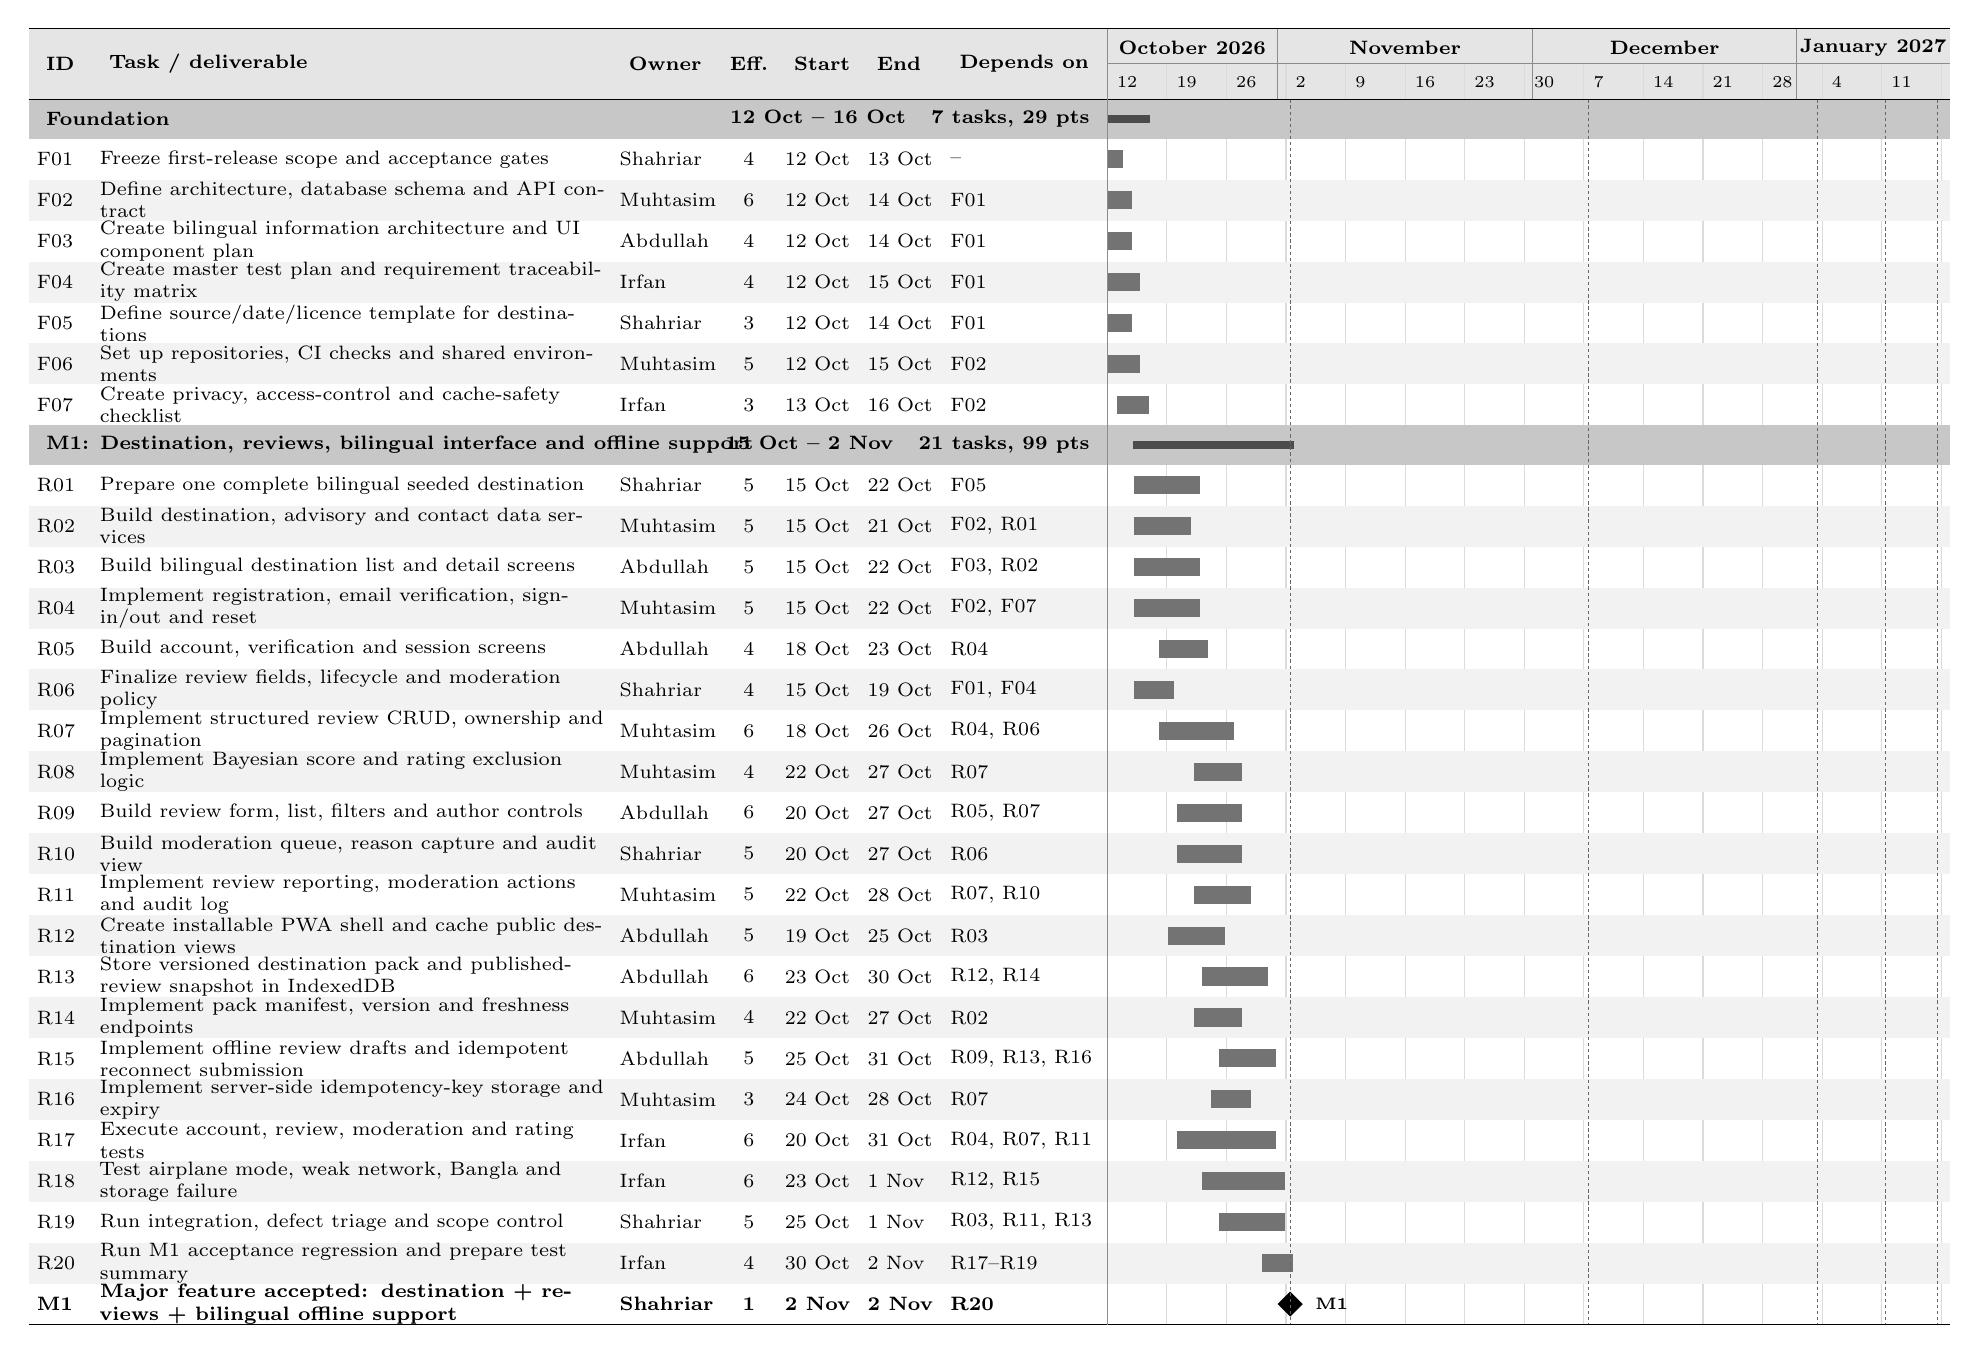
\begin{tikzpicture}[x=1mm,y=-1mm,font=\ganttfont]
\fill[black!10] (0,0) rectangle (244.0,9.0);
\node[anchor=west,font=\ganttfont\bfseries] at (1,4.5) {ID};
\node[anchor=west,font=\ganttfont\bfseries] at (9,4.5) {Task / deliverable};
\node[anchor=west,font=\ganttfont\bfseries] at (75,4.5) {Owner};
\node[anchor=center,font=\ganttfont\bfseries] at (91.5,4.5) {Eff.};
\node[anchor=west,font=\ganttfont\bfseries] at (96,4.5) {Start};
\node[anchor=west,font=\ganttfont\bfseries] at (106.5,4.5) {End};
\node[anchor=west,font=\ganttfont\bfseries] at (117,4.5) {Depends on};
\node[font=\ganttfont\bfseries] at (147.8080808080808,2.43) {October 2026};
\node[font=\ganttfont\bfseries] at (174.82828282828282,2.43) {November};
\draw[black!45] (158.6161616161616,0) -- (158.6161616161616,9.0);
\node[font=\ganttfont\bfseries] at (207.7929292929293,2.43) {December};
\draw[black!45] (191.04040404040404,0) -- (191.04040404040404,9.0);
\node[font=\ganttfont\bfseries] at (234.27272727272728,2.43) {January 2027};
\draw[black!45] (224.54545454545456,0) -- (224.54545454545456,9.0);
\draw[black!45] (137.0,4.5) -- (244.0,4.5);
\node[anchor=west,font=\ganttsmall] at (137.0,6.75) {12};
\node[anchor=west,font=\ganttsmall] at (144.56565656565655,6.75) {19};
\node[anchor=west,font=\ganttsmall] at (152.13131313131314,6.75) {26};
\node[anchor=west,font=\ganttsmall] at (159.6969696969697,6.75) {2};
\node[anchor=west,font=\ganttsmall] at (167.26262626262627,6.75) {9};
\node[anchor=west,font=\ganttsmall] at (174.82828282828282,6.75) {16};
\node[anchor=west,font=\ganttsmall] at (182.3939393939394,6.75) {23};
\node[anchor=west,font=\ganttsmall] at (189.95959595959596,6.75) {30};
\node[anchor=west,font=\ganttsmall] at (197.52525252525254,6.75) {7};
\node[anchor=west,font=\ganttsmall] at (205.0909090909091,6.75) {14};
\node[anchor=west,font=\ganttsmall] at (212.65656565656565,6.75) {21};
\node[anchor=west,font=\ganttsmall] at (220.22222222222223,6.75) {28};
\node[anchor=west,font=\ganttsmall] at (227.7878787878788,6.75) {4};
\node[anchor=west,font=\ganttsmall] at (235.35353535353536,6.75) {11};
\draw[black!14] (144.56565656565655,4.5) -- (144.56565656565655,164.59999999999997);
\draw[black!14] (152.13131313131314,4.5) -- (152.13131313131314,164.59999999999997);
\draw[black!14] (159.6969696969697,4.5) -- (159.6969696969697,164.59999999999997);
\draw[black!14] (167.26262626262627,4.5) -- (167.26262626262627,164.59999999999997);
\draw[black!14] (174.82828282828282,4.5) -- (174.82828282828282,164.59999999999997);
\draw[black!14] (182.3939393939394,4.5) -- (182.3939393939394,164.59999999999997);
\draw[black!14] (189.95959595959596,4.5) -- (189.95959595959596,164.59999999999997);
\draw[black!14] (197.52525252525254,4.5) -- (197.52525252525254,164.59999999999997);
\draw[black!14] (205.0909090909091,4.5) -- (205.0909090909091,164.59999999999997);
\draw[black!14] (212.65656565656565,4.5) -- (212.65656565656565,164.59999999999997);
\draw[black!14] (220.22222222222223,4.5) -- (220.22222222222223,164.59999999999997);
\draw[black!14] (227.7878787878788,4.5) -- (227.7878787878788,164.59999999999997);
\draw[black!14] (235.35353535353536,4.5) -- (235.35353535353536,164.59999999999997);
\draw[black!14] (242.91919191919192,4.5) -- (242.91919191919192,164.59999999999997);
\fill[black!22] (0,9.0) rectangle (244.0,14.0);
\node[anchor=west,font=\ganttfont\bfseries] at (1,11.5) {Foundation};
\node[anchor=east,font=\ganttfont\bfseries] at (136.0,11.5) {12 Oct -- 16 Oct\quad 7 tasks, 29 pts};
\fill[black!70] (137.0,11.0) rectangle (142.40404040404042,12.0);
\node[anchor=west,inner sep=0pt,font=\ganttfont] at (1,16.6) {F01};
\node[anchor=west,text width=64mm,align=left,inner sep=0pt,font=\ganttfont] at (9,16.6) {Freeze first-release scope and acceptance gates};
\node[anchor=west,inner sep=0pt,font=\ganttfont] at (75,16.6) {Shahriar};
\node[anchor=center,inner sep=0pt,font=\ganttfont] at (91.5,16.6) {4};
\node[anchor=west,inner sep=0pt,font=\ganttfont] at (96,16.6) {12 Oct};
\node[anchor=west,inner sep=0pt,font=\ganttfont] at (106.5,16.6) {13 Oct};
\node[anchor=west,inner sep=0pt,font=\ganttfont] at (117,16.6) {--};
\fill[black!55] (137.15,15.450000000000001) rectangle (139.01161616161616,17.75);
\fill[black!5] (0,19.2) rectangle (244.0,24.4);
\node[anchor=west,inner sep=0pt,font=\ganttfont] at (1,21.8) {F02};
\node[anchor=west,text width=64mm,align=left,inner sep=0pt,font=\ganttfont] at (9,21.8) {Define architecture, database schema and API contract};
\node[anchor=west,inner sep=0pt,font=\ganttfont] at (75,21.8) {Muhtasim};
\node[anchor=center,inner sep=0pt,font=\ganttfont] at (91.5,21.8) {6};
\node[anchor=west,inner sep=0pt,font=\ganttfont] at (96,21.8) {12 Oct};
\node[anchor=west,inner sep=0pt,font=\ganttfont] at (106.5,21.8) {14 Oct};
\node[anchor=west,inner sep=0pt,font=\ganttfont] at (117,21.8) {F01};
\fill[black!55] (137.15,20.650000000000002) rectangle (140.09242424242424,22.95);
\node[anchor=west,inner sep=0pt,font=\ganttfont] at (1,27.0) {F03};
\node[anchor=west,text width=64mm,align=left,inner sep=0pt,font=\ganttfont] at (9,27.0) {Create bilingual information architecture and UI component plan};
\node[anchor=west,inner sep=0pt,font=\ganttfont] at (75,27.0) {Abdullah};
\node[anchor=center,inner sep=0pt,font=\ganttfont] at (91.5,27.0) {4};
\node[anchor=west,inner sep=0pt,font=\ganttfont] at (96,27.0) {12 Oct};
\node[anchor=west,inner sep=0pt,font=\ganttfont] at (106.5,27.0) {14 Oct};
\node[anchor=west,inner sep=0pt,font=\ganttfont] at (117,27.0) {F01};
\fill[black!55] (137.15,25.85) rectangle (140.09242424242424,28.15);
\fill[black!5] (0,29.599999999999998) rectangle (244.0,34.8);
\node[anchor=west,inner sep=0pt,font=\ganttfont] at (1,32.199999999999996) {F04};
\node[anchor=west,text width=64mm,align=left,inner sep=0pt,font=\ganttfont] at (9,32.199999999999996) {Create master test plan and requirement traceability matrix};
\node[anchor=west,inner sep=0pt,font=\ganttfont] at (75,32.199999999999996) {Irfan};
\node[anchor=center,inner sep=0pt,font=\ganttfont] at (91.5,32.199999999999996) {4};
\node[anchor=west,inner sep=0pt,font=\ganttfont] at (96,32.199999999999996) {12 Oct};
\node[anchor=west,inner sep=0pt,font=\ganttfont] at (106.5,32.199999999999996) {15 Oct};
\node[anchor=west,inner sep=0pt,font=\ganttfont] at (117,32.199999999999996) {F01};
\fill[black!55] (137.15,31.049999999999997) rectangle (141.17323232323233,33.349999999999994);
\node[anchor=west,inner sep=0pt,font=\ganttfont] at (1,37.4) {F05};
\node[anchor=west,text width=64mm,align=left,inner sep=0pt,font=\ganttfont] at (9,37.4) {Define source/date/licence template for destinations};
\node[anchor=west,inner sep=0pt,font=\ganttfont] at (75,37.4) {Shahriar};
\node[anchor=center,inner sep=0pt,font=\ganttfont] at (91.5,37.4) {3};
\node[anchor=west,inner sep=0pt,font=\ganttfont] at (96,37.4) {12 Oct};
\node[anchor=west,inner sep=0pt,font=\ganttfont] at (106.5,37.4) {14 Oct};
\node[anchor=west,inner sep=0pt,font=\ganttfont] at (117,37.4) {F01};
\fill[black!55] (137.15,36.25) rectangle (140.09242424242424,38.55);
\fill[black!5] (0,40.0) rectangle (244.0,45.2);
\node[anchor=west,inner sep=0pt,font=\ganttfont] at (1,42.6) {F06};
\node[anchor=west,text width=64mm,align=left,inner sep=0pt,font=\ganttfont] at (9,42.6) {Set up repositories, CI checks and shared environments};
\node[anchor=west,inner sep=0pt,font=\ganttfont] at (75,42.6) {Muhtasim};
\node[anchor=center,inner sep=0pt,font=\ganttfont] at (91.5,42.6) {5};
\node[anchor=west,inner sep=0pt,font=\ganttfont] at (96,42.6) {12 Oct};
\node[anchor=west,inner sep=0pt,font=\ganttfont] at (106.5,42.6) {15 Oct};
\node[anchor=west,inner sep=0pt,font=\ganttfont] at (117,42.6) {F02};
\fill[black!55] (137.15,41.45) rectangle (141.17323232323233,43.75);
\node[anchor=west,inner sep=0pt,font=\ganttfont] at (1,47.800000000000004) {F07};
\node[anchor=west,text width=64mm,align=left,inner sep=0pt,font=\ganttfont] at (9,47.800000000000004) {Create privacy, access-control and cache-safety checklist};
\node[anchor=west,inner sep=0pt,font=\ganttfont] at (75,47.800000000000004) {Irfan};
\node[anchor=center,inner sep=0pt,font=\ganttfont] at (91.5,47.800000000000004) {3};
\node[anchor=west,inner sep=0pt,font=\ganttfont] at (96,47.800000000000004) {13 Oct};
\node[anchor=west,inner sep=0pt,font=\ganttfont] at (106.5,47.800000000000004) {16 Oct};
\node[anchor=west,inner sep=0pt,font=\ganttfont] at (117,47.800000000000004) {F02};
\fill[black!55] (138.2308080808081,46.650000000000006) rectangle (142.2540404040404,48.95);
\fill[black!22] (0,50.400000000000006) rectangle (244.0,55.400000000000006);
\node[anchor=west,font=\ganttfont\bfseries] at (1,52.900000000000006) {M1: Destination, reviews, bilingual interface and offline support};
\node[anchor=east,font=\ganttfont\bfseries] at (136.0,52.900000000000006) {15 Oct -- 2 Nov\quad 21 tasks, 99 pts};
\fill[black!70] (140.24242424242425,52.400000000000006) rectangle (160.77777777777777,53.400000000000006);
\node[anchor=west,inner sep=0pt,font=\ganttfont] at (1,58.00000000000001) {R01};
\node[anchor=west,text width=64mm,align=left,inner sep=0pt,font=\ganttfont] at (9,58.00000000000001) {Prepare one complete bilingual seeded destination};
\node[anchor=west,inner sep=0pt,font=\ganttfont] at (75,58.00000000000001) {Shahriar};
\node[anchor=center,inner sep=0pt,font=\ganttfont] at (91.5,58.00000000000001) {5};
\node[anchor=west,inner sep=0pt,font=\ganttfont] at (96,58.00000000000001) {15 Oct};
\node[anchor=west,inner sep=0pt,font=\ganttfont] at (106.5,58.00000000000001) {22 Oct};
\node[anchor=west,inner sep=0pt,font=\ganttfont] at (117,58.00000000000001) {F05};
\fill[black!55] (140.39242424242425,56.85000000000001) rectangle (148.73888888888888,59.150000000000006);
\fill[black!5] (0,60.60000000000001) rectangle (244.0,65.80000000000001);
\node[anchor=west,inner sep=0pt,font=\ganttfont] at (1,63.20000000000001) {R02};
\node[anchor=west,text width=64mm,align=left,inner sep=0pt,font=\ganttfont] at (9,63.20000000000001) {Build destination, advisory and contact data services};
\node[anchor=west,inner sep=0pt,font=\ganttfont] at (75,63.20000000000001) {Muhtasim};
\node[anchor=center,inner sep=0pt,font=\ganttfont] at (91.5,63.20000000000001) {5};
\node[anchor=west,inner sep=0pt,font=\ganttfont] at (96,63.20000000000001) {15 Oct};
\node[anchor=west,inner sep=0pt,font=\ganttfont] at (106.5,63.20000000000001) {21 Oct};
\node[anchor=west,inner sep=0pt,font=\ganttfont] at (117,63.20000000000001) {F02, R01};
\fill[black!55] (140.39242424242425,62.05000000000001) rectangle (147.6580808080808,64.35000000000001);
\node[anchor=west,inner sep=0pt,font=\ganttfont] at (1,68.4) {R03};
\node[anchor=west,text width=64mm,align=left,inner sep=0pt,font=\ganttfont] at (9,68.4) {Build bilingual destination list and detail screens};
\node[anchor=west,inner sep=0pt,font=\ganttfont] at (75,68.4) {Abdullah};
\node[anchor=center,inner sep=0pt,font=\ganttfont] at (91.5,68.4) {5};
\node[anchor=west,inner sep=0pt,font=\ganttfont] at (96,68.4) {15 Oct};
\node[anchor=west,inner sep=0pt,font=\ganttfont] at (106.5,68.4) {22 Oct};
\node[anchor=west,inner sep=0pt,font=\ganttfont] at (117,68.4) {F03, R02};
\fill[black!55] (140.39242424242425,67.25) rectangle (148.73888888888888,69.55000000000001);
\fill[black!5] (0,71.00000000000001) rectangle (244.0,76.20000000000002);
\node[anchor=west,inner sep=0pt,font=\ganttfont] at (1,73.60000000000001) {R04};
\node[anchor=west,text width=64mm,align=left,inner sep=0pt,font=\ganttfont] at (9,73.60000000000001) {Implement registration, email verification, sign-in/out and reset};
\node[anchor=west,inner sep=0pt,font=\ganttfont] at (75,73.60000000000001) {Muhtasim};
\node[anchor=center,inner sep=0pt,font=\ganttfont] at (91.5,73.60000000000001) {5};
\node[anchor=west,inner sep=0pt,font=\ganttfont] at (96,73.60000000000001) {15 Oct};
\node[anchor=west,inner sep=0pt,font=\ganttfont] at (106.5,73.60000000000001) {22 Oct};
\node[anchor=west,inner sep=0pt,font=\ganttfont] at (117,73.60000000000001) {F02, F07};
\fill[black!55] (140.39242424242425,72.45) rectangle (148.73888888888888,74.75000000000001);
\node[anchor=west,inner sep=0pt,font=\ganttfont] at (1,78.80000000000001) {R05};
\node[anchor=west,text width=64mm,align=left,inner sep=0pt,font=\ganttfont] at (9,78.80000000000001) {Build account, verification and session screens};
\node[anchor=west,inner sep=0pt,font=\ganttfont] at (75,78.80000000000001) {Abdullah};
\node[anchor=center,inner sep=0pt,font=\ganttfont] at (91.5,78.80000000000001) {4};
\node[anchor=west,inner sep=0pt,font=\ganttfont] at (96,78.80000000000001) {18 Oct};
\node[anchor=west,inner sep=0pt,font=\ganttfont] at (106.5,78.80000000000001) {23 Oct};
\node[anchor=west,inner sep=0pt,font=\ganttfont] at (117,78.80000000000001) {R04};
\fill[black!55] (143.6348484848485,77.65) rectangle (149.81969696969696,79.95000000000002);
\fill[black!5] (0,81.40000000000002) rectangle (244.0,86.60000000000002);
\node[anchor=west,inner sep=0pt,font=\ganttfont] at (1,84.00000000000001) {R06};
\node[anchor=west,text width=64mm,align=left,inner sep=0pt,font=\ganttfont] at (9,84.00000000000001) {Finalize review fields, lifecycle and moderation policy};
\node[anchor=west,inner sep=0pt,font=\ganttfont] at (75,84.00000000000001) {Shahriar};
\node[anchor=center,inner sep=0pt,font=\ganttfont] at (91.5,84.00000000000001) {4};
\node[anchor=west,inner sep=0pt,font=\ganttfont] at (96,84.00000000000001) {15 Oct};
\node[anchor=west,inner sep=0pt,font=\ganttfont] at (106.5,84.00000000000001) {19 Oct};
\node[anchor=west,inner sep=0pt,font=\ganttfont] at (117,84.00000000000001) {F01, F04};
\fill[black!55] (140.39242424242425,82.85000000000001) rectangle (145.49646464646463,85.15000000000002);
\node[anchor=west,inner sep=0pt,font=\ganttfont] at (1,89.20000000000002) {R07};
\node[anchor=west,text width=64mm,align=left,inner sep=0pt,font=\ganttfont] at (9,89.20000000000002) {Implement structured review CRUD, ownership and pagination};
\node[anchor=west,inner sep=0pt,font=\ganttfont] at (75,89.20000000000002) {Muhtasim};
\node[anchor=center,inner sep=0pt,font=\ganttfont] at (91.5,89.20000000000002) {6};
\node[anchor=west,inner sep=0pt,font=\ganttfont] at (96,89.20000000000002) {18 Oct};
\node[anchor=west,inner sep=0pt,font=\ganttfont] at (106.5,89.20000000000002) {26 Oct};
\node[anchor=west,inner sep=0pt,font=\ganttfont] at (117,89.20000000000002) {R04, R06};
\fill[black!55] (143.6348484848485,88.05000000000001) rectangle (153.0621212121212,90.35000000000002);
\fill[black!5] (0,91.80000000000003) rectangle (244.0,97.00000000000003);
\node[anchor=west,inner sep=0pt,font=\ganttfont] at (1,94.40000000000002) {R08};
\node[anchor=west,text width=64mm,align=left,inner sep=0pt,font=\ganttfont] at (9,94.40000000000002) {Implement Bayesian score and rating exclusion logic};
\node[anchor=west,inner sep=0pt,font=\ganttfont] at (75,94.40000000000002) {Muhtasim};
\node[anchor=center,inner sep=0pt,font=\ganttfont] at (91.5,94.40000000000002) {4};
\node[anchor=west,inner sep=0pt,font=\ganttfont] at (96,94.40000000000002) {22 Oct};
\node[anchor=west,inner sep=0pt,font=\ganttfont] at (106.5,94.40000000000002) {27 Oct};
\node[anchor=west,inner sep=0pt,font=\ganttfont] at (117,94.40000000000002) {R07};
\fill[black!55] (147.9580808080808,93.25000000000001) rectangle (154.1429292929293,95.55000000000003);
\node[anchor=west,inner sep=0pt,font=\ganttfont] at (1,99.60000000000002) {R09};
\node[anchor=west,text width=64mm,align=left,inner sep=0pt,font=\ganttfont] at (9,99.60000000000002) {Build review form, list, filters and author controls};
\node[anchor=west,inner sep=0pt,font=\ganttfont] at (75,99.60000000000002) {Abdullah};
\node[anchor=center,inner sep=0pt,font=\ganttfont] at (91.5,99.60000000000002) {6};
\node[anchor=west,inner sep=0pt,font=\ganttfont] at (96,99.60000000000002) {20 Oct};
\node[anchor=west,inner sep=0pt,font=\ganttfont] at (106.5,99.60000000000002) {27 Oct};
\node[anchor=west,inner sep=0pt,font=\ganttfont] at (117,99.60000000000002) {R05, R07};
\fill[black!55] (145.79646464646464,98.45000000000002) rectangle (154.1429292929293,100.75000000000003);
\fill[black!5] (0,102.20000000000003) rectangle (244.0,107.40000000000003);
\node[anchor=west,inner sep=0pt,font=\ganttfont] at (1,104.80000000000003) {R10};
\node[anchor=west,text width=64mm,align=left,inner sep=0pt,font=\ganttfont] at (9,104.80000000000003) {Build moderation queue, reason capture and audit view};
\node[anchor=west,inner sep=0pt,font=\ganttfont] at (75,104.80000000000003) {Shahriar};
\node[anchor=center,inner sep=0pt,font=\ganttfont] at (91.5,104.80000000000003) {5};
\node[anchor=west,inner sep=0pt,font=\ganttfont] at (96,104.80000000000003) {20 Oct};
\node[anchor=west,inner sep=0pt,font=\ganttfont] at (106.5,104.80000000000003) {27 Oct};
\node[anchor=west,inner sep=0pt,font=\ganttfont] at (117,104.80000000000003) {R06};
\fill[black!55] (145.79646464646464,103.65000000000002) rectangle (154.1429292929293,105.95000000000003);
\node[anchor=west,inner sep=0pt,font=\ganttfont] at (1,110.00000000000003) {R11};
\node[anchor=west,text width=64mm,align=left,inner sep=0pt,font=\ganttfont] at (9,110.00000000000003) {Implement review reporting, moderation actions and audit log};
\node[anchor=west,inner sep=0pt,font=\ganttfont] at (75,110.00000000000003) {Muhtasim};
\node[anchor=center,inner sep=0pt,font=\ganttfont] at (91.5,110.00000000000003) {5};
\node[anchor=west,inner sep=0pt,font=\ganttfont] at (96,110.00000000000003) {22 Oct};
\node[anchor=west,inner sep=0pt,font=\ganttfont] at (106.5,110.00000000000003) {28 Oct};
\node[anchor=west,inner sep=0pt,font=\ganttfont] at (117,110.00000000000003) {R07, R10};
\fill[black!55] (147.9580808080808,108.85000000000002) rectangle (155.22373737373738,111.15000000000003);
\fill[black!5] (0,112.60000000000004) rectangle (244.0,117.80000000000004);
\node[anchor=west,inner sep=0pt,font=\ganttfont] at (1,115.20000000000003) {R12};
\node[anchor=west,text width=64mm,align=left,inner sep=0pt,font=\ganttfont] at (9,115.20000000000003) {Create installable PWA shell and cache public destination views};
\node[anchor=west,inner sep=0pt,font=\ganttfont] at (75,115.20000000000003) {Abdullah};
\node[anchor=center,inner sep=0pt,font=\ganttfont] at (91.5,115.20000000000003) {5};
\node[anchor=west,inner sep=0pt,font=\ganttfont] at (96,115.20000000000003) {19 Oct};
\node[anchor=west,inner sep=0pt,font=\ganttfont] at (106.5,115.20000000000003) {25 Oct};
\node[anchor=west,inner sep=0pt,font=\ganttfont] at (117,115.20000000000003) {R03};
\fill[black!55] (144.71565656565656,114.05000000000003) rectangle (151.98131313131313,116.35000000000004);
\node[anchor=west,inner sep=0pt,font=\ganttfont] at (1,120.40000000000003) {R13};
\node[anchor=west,text width=64mm,align=left,inner sep=0pt,font=\ganttfont] at (9,120.40000000000003) {Store versioned destination pack and published-review snapshot in IndexedDB};
\node[anchor=west,inner sep=0pt,font=\ganttfont] at (75,120.40000000000003) {Abdullah};
\node[anchor=center,inner sep=0pt,font=\ganttfont] at (91.5,120.40000000000003) {6};
\node[anchor=west,inner sep=0pt,font=\ganttfont] at (96,120.40000000000003) {23 Oct};
\node[anchor=west,inner sep=0pt,font=\ganttfont] at (106.5,120.40000000000003) {30 Oct};
\node[anchor=west,inner sep=0pt,font=\ganttfont] at (117,120.40000000000003) {R12, R14};
\fill[black!55] (149.0388888888889,119.25000000000003) rectangle (157.38535353535354,121.55000000000004);
\fill[black!5] (0,123.00000000000004) rectangle (244.0,128.20000000000005);
\node[anchor=west,inner sep=0pt,font=\ganttfont] at (1,125.60000000000004) {R14};
\node[anchor=west,text width=64mm,align=left,inner sep=0pt,font=\ganttfont] at (9,125.60000000000004) {Implement pack manifest, version and freshness endpoints};
\node[anchor=west,inner sep=0pt,font=\ganttfont] at (75,125.60000000000004) {Muhtasim};
\node[anchor=center,inner sep=0pt,font=\ganttfont] at (91.5,125.60000000000004) {4};
\node[anchor=west,inner sep=0pt,font=\ganttfont] at (96,125.60000000000004) {22 Oct};
\node[anchor=west,inner sep=0pt,font=\ganttfont] at (106.5,125.60000000000004) {27 Oct};
\node[anchor=west,inner sep=0pt,font=\ganttfont] at (117,125.60000000000004) {R02};
\fill[black!55] (147.9580808080808,124.45000000000003) rectangle (154.1429292929293,126.75000000000004);
\node[anchor=west,inner sep=0pt,font=\ganttfont] at (1,130.80000000000004) {R15};
\node[anchor=west,text width=64mm,align=left,inner sep=0pt,font=\ganttfont] at (9,130.80000000000004) {Implement offline review drafts and idempotent reconnect submission};
\node[anchor=west,inner sep=0pt,font=\ganttfont] at (75,130.80000000000004) {Abdullah};
\node[anchor=center,inner sep=0pt,font=\ganttfont] at (91.5,130.80000000000004) {5};
\node[anchor=west,inner sep=0pt,font=\ganttfont] at (96,130.80000000000004) {25 Oct};
\node[anchor=west,inner sep=0pt,font=\ganttfont] at (106.5,130.80000000000004) {31 Oct};
\node[anchor=west,inner sep=0pt,font=\ganttfont] at (117,130.80000000000004) {R09, R13, R16};
\fill[black!55] (151.20050505050506,129.65000000000003) rectangle (158.4661616161616,131.95000000000005);
\fill[black!5] (0,133.40000000000003) rectangle (244.0,138.60000000000002);
\node[anchor=west,inner sep=0pt,font=\ganttfont] at (1,136.00000000000003) {R16};
\node[anchor=west,text width=64mm,align=left,inner sep=0pt,font=\ganttfont] at (9,136.00000000000003) {Implement server-side idempotency-key storage and expiry};
\node[anchor=west,inner sep=0pt,font=\ganttfont] at (75,136.00000000000003) {Muhtasim};
\node[anchor=center,inner sep=0pt,font=\ganttfont] at (91.5,136.00000000000003) {3};
\node[anchor=west,inner sep=0pt,font=\ganttfont] at (96,136.00000000000003) {24 Oct};
\node[anchor=west,inner sep=0pt,font=\ganttfont] at (106.5,136.00000000000003) {28 Oct};
\node[anchor=west,inner sep=0pt,font=\ganttfont] at (117,136.00000000000003) {R07};
\fill[black!55] (150.11969696969697,134.85000000000002) rectangle (155.22373737373738,137.15000000000003);
\node[anchor=west,inner sep=0pt,font=\ganttfont] at (1,141.20000000000002) {R17};
\node[anchor=west,text width=64mm,align=left,inner sep=0pt,font=\ganttfont] at (9,141.20000000000002) {Execute account, review, moderation and rating tests};
\node[anchor=west,inner sep=0pt,font=\ganttfont] at (75,141.20000000000002) {Irfan};
\node[anchor=center,inner sep=0pt,font=\ganttfont] at (91.5,141.20000000000002) {6};
\node[anchor=west,inner sep=0pt,font=\ganttfont] at (96,141.20000000000002) {20 Oct};
\node[anchor=west,inner sep=0pt,font=\ganttfont] at (106.5,141.20000000000002) {31 Oct};
\node[anchor=west,inner sep=0pt,font=\ganttfont] at (117,141.20000000000002) {R04, R07, R11};
\fill[black!55] (145.79646464646464,140.05) rectangle (158.4661616161616,142.35000000000002);
\fill[black!5] (0,143.8) rectangle (244.0,149.0);
\node[anchor=west,inner sep=0pt,font=\ganttfont] at (1,146.4) {R18};
\node[anchor=west,text width=64mm,align=left,inner sep=0pt,font=\ganttfont] at (9,146.4) {Test airplane mode, weak network, Bangla and storage failure};
\node[anchor=west,inner sep=0pt,font=\ganttfont] at (75,146.4) {Irfan};
\node[anchor=center,inner sep=0pt,font=\ganttfont] at (91.5,146.4) {6};
\node[anchor=west,inner sep=0pt,font=\ganttfont] at (96,146.4) {23 Oct};
\node[anchor=west,inner sep=0pt,font=\ganttfont] at (106.5,146.4) {1 Nov};
\node[anchor=west,inner sep=0pt,font=\ganttfont] at (117,146.4) {R12, R15};
\fill[black!55] (149.0388888888889,145.25) rectangle (159.54696969696968,147.55);
\node[anchor=west,inner sep=0pt,font=\ganttfont] at (1,151.6) {R19};
\node[anchor=west,text width=64mm,align=left,inner sep=0pt,font=\ganttfont] at (9,151.6) {Run integration, defect triage and scope control};
\node[anchor=west,inner sep=0pt,font=\ganttfont] at (75,151.6) {Shahriar};
\node[anchor=center,inner sep=0pt,font=\ganttfont] at (91.5,151.6) {5};
\node[anchor=west,inner sep=0pt,font=\ganttfont] at (96,151.6) {25 Oct};
\node[anchor=west,inner sep=0pt,font=\ganttfont] at (106.5,151.6) {1 Nov};
\node[anchor=west,inner sep=0pt,font=\ganttfont] at (117,151.6) {R03, R11, R13};
\fill[black!55] (151.20050505050506,150.45) rectangle (159.54696969696968,152.75);
\fill[black!5] (0,154.2) rectangle (244.0,159.39999999999998);
\node[anchor=west,inner sep=0pt,font=\ganttfont] at (1,156.79999999999998) {R20};
\node[anchor=west,text width=64mm,align=left,inner sep=0pt,font=\ganttfont] at (9,156.79999999999998) {Run M1 acceptance regression and prepare test summary};
\node[anchor=west,inner sep=0pt,font=\ganttfont] at (75,156.79999999999998) {Irfan};
\node[anchor=center,inner sep=0pt,font=\ganttfont] at (91.5,156.79999999999998) {4};
\node[anchor=west,inner sep=0pt,font=\ganttfont] at (96,156.79999999999998) {30 Oct};
\node[anchor=west,inner sep=0pt,font=\ganttfont] at (106.5,156.79999999999998) {2 Nov};
\node[anchor=west,inner sep=0pt,font=\ganttfont] at (117,156.79999999999998) {R17--R19};
\fill[black!55] (156.60454545454547,155.64999999999998) rectangle (160.62777777777777,157.95);
\node[anchor=west,inner sep=0pt,font=\ganttfont\bfseries] at (1,161.99999999999997) {M1};
\node[anchor=west,text width=64mm,align=left,inner sep=0pt,font=\ganttfont\bfseries] at (9,161.99999999999997) {Major feature accepted: destination + reviews + bilingual offline support};
\node[anchor=west,inner sep=0pt,font=\ganttfont\bfseries] at (75,161.99999999999997) {Shahriar};
\node[anchor=center,inner sep=0pt,font=\ganttfont\bfseries] at (91.5,161.99999999999997) {1};
\node[anchor=west,inner sep=0pt,font=\ganttfont\bfseries] at (96,161.99999999999997) {2 Nov};
\node[anchor=west,inner sep=0pt,font=\ganttfont\bfseries] at (106.5,161.99999999999997) {2 Nov};
\node[anchor=west,inner sep=0pt,font=\ganttfont\bfseries] at (117,161.99999999999997) {R20};
\fill[black] (160.23737373737373,160.39999999999998) -- (161.83737373737372,161.99999999999997) -- (160.23737373737373,163.59999999999997) -- (158.63737373737374,161.99999999999997) -- cycle;
\node[anchor=west,font=\ganttsmall\bfseries] at (162.17777777777778,161.99999999999997) {M1};
\draw[black!60,dash pattern=on 1.2pt off 1pt,line width=0.35pt] (160.23737373737373,9.0) -- (160.23737373737373,164.59999999999997);
\draw[black!60,dash pattern=on 1.2pt off 1pt,line width=0.35pt] (198.06565656565658,9.0) -- (198.06565656565658,164.59999999999997);
\draw[black!60,dash pattern=on 1.2pt off 1pt,line width=0.35pt] (227.24747474747477,9.0) -- (227.24747474747477,164.59999999999997);
\draw[black!60,dash pattern=on 1.2pt off 1pt,line width=0.35pt] (235.8939393939394,9.0) -- (235.8939393939394,164.59999999999997);
\draw[black!60,dash pattern=on 1.2pt off 1pt,line width=0.35pt] (242.37878787878788,9.0) -- (242.37878787878788,164.59999999999997);
\draw[line width=0.6pt] (0,0) -- (244.0,0);
\draw[line width=0.4pt] (0,9.0) -- (244.0,9.0);
\draw[line width=0.6pt] (0,164.59999999999997) -- (244.0,164.59999999999997);
\draw[black!45] (137.0,0) -- (137.0,164.59999999999997);
\end{tikzpicture}
}
\end{minipage}
\clearpage
\thispagestyle{plain}
\vspace*{-10mm}
\noindent\begin{minipage}[b][150mm][t]{\linewidth}\centering
\captionof{figure}{Implementation Gantt chart, part 2 of 3: cost estimator, 50--60\% checkpoint (M2), and hardening}\label{fig:gantt2}
\vspace{-1mm}
{\small Live schedule: \extlink{https://docs.google.com/spreadsheets/d/1efTW9JKtYhHZKrualfaJKGMggvZNjNmESuBnQbCRPiQ/edit?gid=1652090786\#gid=1652090786}{open the Gantt chart in Google Sheets}\par}
\vspace{1.5mm}
\makebox[\linewidth][c]{%
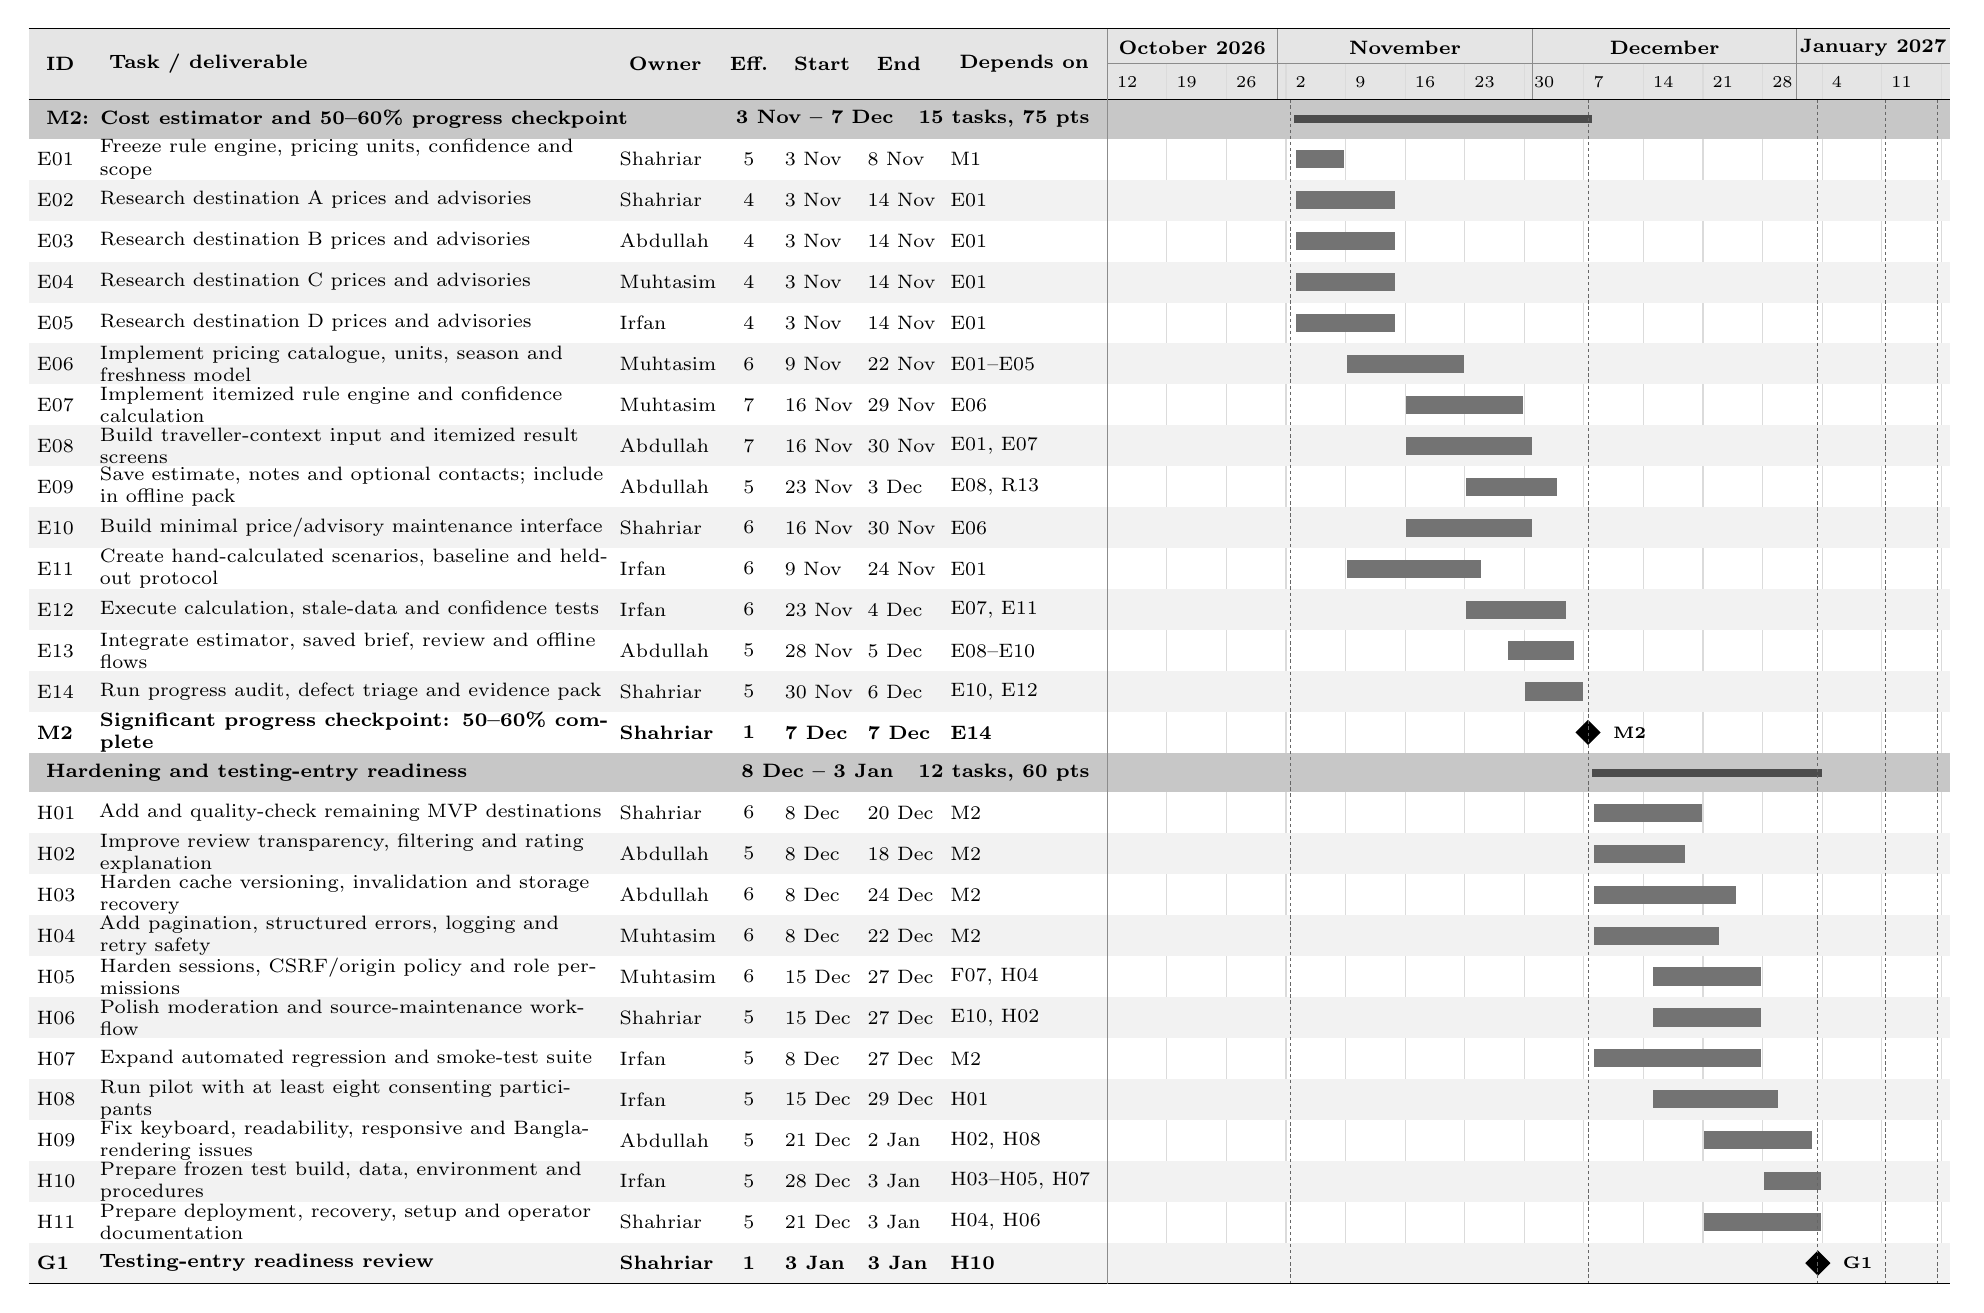
\begin{tikzpicture}[x=1mm,y=-1mm,font=\ganttfont]
\fill[black!10] (0,0) rectangle (244.0,9.0);
\node[anchor=west,font=\ganttfont\bfseries] at (1,4.5) {ID};
\node[anchor=west,font=\ganttfont\bfseries] at (9,4.5) {Task / deliverable};
\node[anchor=west,font=\ganttfont\bfseries] at (75,4.5) {Owner};
\node[anchor=center,font=\ganttfont\bfseries] at (91.5,4.5) {Eff.};
\node[anchor=west,font=\ganttfont\bfseries] at (96,4.5) {Start};
\node[anchor=west,font=\ganttfont\bfseries] at (106.5,4.5) {End};
\node[anchor=west,font=\ganttfont\bfseries] at (117,4.5) {Depends on};
\node[font=\ganttfont\bfseries] at (147.8080808080808,2.43) {October 2026};
\node[font=\ganttfont\bfseries] at (174.82828282828282,2.43) {November};
\draw[black!45] (158.6161616161616,0) -- (158.6161616161616,9.0);
\node[font=\ganttfont\bfseries] at (207.7929292929293,2.43) {December};
\draw[black!45] (191.04040404040404,0) -- (191.04040404040404,9.0);
\node[font=\ganttfont\bfseries] at (234.27272727272728,2.43) {January 2027};
\draw[black!45] (224.54545454545456,0) -- (224.54545454545456,9.0);
\draw[black!45] (137.0,4.5) -- (244.0,4.5);
\node[anchor=west,font=\ganttsmall] at (137.0,6.75) {12};
\node[anchor=west,font=\ganttsmall] at (144.56565656565655,6.75) {19};
\node[anchor=west,font=\ganttsmall] at (152.13131313131314,6.75) {26};
\node[anchor=west,font=\ganttsmall] at (159.6969696969697,6.75) {2};
\node[anchor=west,font=\ganttsmall] at (167.26262626262627,6.75) {9};
\node[anchor=west,font=\ganttsmall] at (174.82828282828282,6.75) {16};
\node[anchor=west,font=\ganttsmall] at (182.3939393939394,6.75) {23};
\node[anchor=west,font=\ganttsmall] at (189.95959595959596,6.75) {30};
\node[anchor=west,font=\ganttsmall] at (197.52525252525254,6.75) {7};
\node[anchor=west,font=\ganttsmall] at (205.0909090909091,6.75) {14};
\node[anchor=west,font=\ganttsmall] at (212.65656565656565,6.75) {21};
\node[anchor=west,font=\ganttsmall] at (220.22222222222223,6.75) {28};
\node[anchor=west,font=\ganttsmall] at (227.7878787878788,6.75) {4};
\node[anchor=west,font=\ganttsmall] at (235.35353535353536,6.75) {11};
\draw[black!14] (144.56565656565655,4.5) -- (144.56565656565655,159.39999999999998);
\draw[black!14] (152.13131313131314,4.5) -- (152.13131313131314,159.39999999999998);
\draw[black!14] (159.6969696969697,4.5) -- (159.6969696969697,159.39999999999998);
\draw[black!14] (167.26262626262627,4.5) -- (167.26262626262627,159.39999999999998);
\draw[black!14] (174.82828282828282,4.5) -- (174.82828282828282,159.39999999999998);
\draw[black!14] (182.3939393939394,4.5) -- (182.3939393939394,159.39999999999998);
\draw[black!14] (189.95959595959596,4.5) -- (189.95959595959596,159.39999999999998);
\draw[black!14] (197.52525252525254,4.5) -- (197.52525252525254,159.39999999999998);
\draw[black!14] (205.0909090909091,4.5) -- (205.0909090909091,159.39999999999998);
\draw[black!14] (212.65656565656565,4.5) -- (212.65656565656565,159.39999999999998);
\draw[black!14] (220.22222222222223,4.5) -- (220.22222222222223,159.39999999999998);
\draw[black!14] (227.7878787878788,4.5) -- (227.7878787878788,159.39999999999998);
\draw[black!14] (235.35353535353536,4.5) -- (235.35353535353536,159.39999999999998);
\draw[black!14] (242.91919191919192,4.5) -- (242.91919191919192,159.39999999999998);
\fill[black!22] (0,9.0) rectangle (244.0,14.0);
\node[anchor=west,font=\ganttfont\bfseries] at (1,11.5) {M2: Cost estimator and 50--60\% progress checkpoint};
\node[anchor=east,font=\ganttfont\bfseries] at (136.0,11.5) {3 Nov -- 7 Dec\quad 15 tasks, 75 pts};
\fill[black!70] (160.77777777777777,11.0) rectangle (198.60606060606062,12.0);
\node[anchor=west,inner sep=0pt,font=\ganttfont] at (1,16.6) {E01};
\node[anchor=west,text width=64mm,align=left,inner sep=0pt,font=\ganttfont] at (9,16.6) {Freeze rule engine, pricing units, confidence and scope};
\node[anchor=west,inner sep=0pt,font=\ganttfont] at (75,16.6) {Shahriar};
\node[anchor=center,inner sep=0pt,font=\ganttfont] at (91.5,16.6) {5};
\node[anchor=west,inner sep=0pt,font=\ganttfont] at (96,16.6) {3 Nov};
\node[anchor=west,inner sep=0pt,font=\ganttfont] at (106.5,16.6) {8 Nov};
\node[anchor=west,inner sep=0pt,font=\ganttfont] at (117,16.6) {M1};
\fill[black!55] (160.92777777777778,15.450000000000001) rectangle (167.11262626262626,17.75);
\fill[black!5] (0,19.2) rectangle (244.0,24.4);
\node[anchor=west,inner sep=0pt,font=\ganttfont] at (1,21.8) {E02};
\node[anchor=west,text width=64mm,align=left,inner sep=0pt,font=\ganttfont] at (9,21.8) {Research destination A prices and advisories};
\node[anchor=west,inner sep=0pt,font=\ganttfont] at (75,21.8) {Shahriar};
\node[anchor=center,inner sep=0pt,font=\ganttfont] at (91.5,21.8) {4};
\node[anchor=west,inner sep=0pt,font=\ganttfont] at (96,21.8) {3 Nov};
\node[anchor=west,inner sep=0pt,font=\ganttfont] at (106.5,21.8) {14 Nov};
\node[anchor=west,inner sep=0pt,font=\ganttfont] at (117,21.8) {E01};
\fill[black!55] (160.92777777777778,20.650000000000002) rectangle (173.59747474747476,22.95);
\node[anchor=west,inner sep=0pt,font=\ganttfont] at (1,27.0) {E03};
\node[anchor=west,text width=64mm,align=left,inner sep=0pt,font=\ganttfont] at (9,27.0) {Research destination B prices and advisories};
\node[anchor=west,inner sep=0pt,font=\ganttfont] at (75,27.0) {Abdullah};
\node[anchor=center,inner sep=0pt,font=\ganttfont] at (91.5,27.0) {4};
\node[anchor=west,inner sep=0pt,font=\ganttfont] at (96,27.0) {3 Nov};
\node[anchor=west,inner sep=0pt,font=\ganttfont] at (106.5,27.0) {14 Nov};
\node[anchor=west,inner sep=0pt,font=\ganttfont] at (117,27.0) {E01};
\fill[black!55] (160.92777777777778,25.85) rectangle (173.59747474747476,28.15);
\fill[black!5] (0,29.599999999999998) rectangle (244.0,34.8);
\node[anchor=west,inner sep=0pt,font=\ganttfont] at (1,32.199999999999996) {E04};
\node[anchor=west,text width=64mm,align=left,inner sep=0pt,font=\ganttfont] at (9,32.199999999999996) {Research destination C prices and advisories};
\node[anchor=west,inner sep=0pt,font=\ganttfont] at (75,32.199999999999996) {Muhtasim};
\node[anchor=center,inner sep=0pt,font=\ganttfont] at (91.5,32.199999999999996) {4};
\node[anchor=west,inner sep=0pt,font=\ganttfont] at (96,32.199999999999996) {3 Nov};
\node[anchor=west,inner sep=0pt,font=\ganttfont] at (106.5,32.199999999999996) {14 Nov};
\node[anchor=west,inner sep=0pt,font=\ganttfont] at (117,32.199999999999996) {E01};
\fill[black!55] (160.92777777777778,31.049999999999997) rectangle (173.59747474747476,33.349999999999994);
\node[anchor=west,inner sep=0pt,font=\ganttfont] at (1,37.4) {E05};
\node[anchor=west,text width=64mm,align=left,inner sep=0pt,font=\ganttfont] at (9,37.4) {Research destination D prices and advisories};
\node[anchor=west,inner sep=0pt,font=\ganttfont] at (75,37.4) {Irfan};
\node[anchor=center,inner sep=0pt,font=\ganttfont] at (91.5,37.4) {4};
\node[anchor=west,inner sep=0pt,font=\ganttfont] at (96,37.4) {3 Nov};
\node[anchor=west,inner sep=0pt,font=\ganttfont] at (106.5,37.4) {14 Nov};
\node[anchor=west,inner sep=0pt,font=\ganttfont] at (117,37.4) {E01};
\fill[black!55] (160.92777777777778,36.25) rectangle (173.59747474747476,38.55);
\fill[black!5] (0,40.0) rectangle (244.0,45.2);
\node[anchor=west,inner sep=0pt,font=\ganttfont] at (1,42.6) {E06};
\node[anchor=west,text width=64mm,align=left,inner sep=0pt,font=\ganttfont] at (9,42.6) {Implement pricing catalogue, units, season and freshness model};
\node[anchor=west,inner sep=0pt,font=\ganttfont] at (75,42.6) {Muhtasim};
\node[anchor=center,inner sep=0pt,font=\ganttfont] at (91.5,42.6) {6};
\node[anchor=west,inner sep=0pt,font=\ganttfont] at (96,42.6) {9 Nov};
\node[anchor=west,inner sep=0pt,font=\ganttfont] at (106.5,42.6) {22 Nov};
\node[anchor=west,inner sep=0pt,font=\ganttfont] at (117,42.6) {E01--E05};
\fill[black!55] (167.41262626262628,41.45) rectangle (182.2439393939394,43.75);
\node[anchor=west,inner sep=0pt,font=\ganttfont] at (1,47.800000000000004) {E07};
\node[anchor=west,text width=64mm,align=left,inner sep=0pt,font=\ganttfont] at (9,47.800000000000004) {Implement itemized rule engine and confidence calculation};
\node[anchor=west,inner sep=0pt,font=\ganttfont] at (75,47.800000000000004) {Muhtasim};
\node[anchor=center,inner sep=0pt,font=\ganttfont] at (91.5,47.800000000000004) {7};
\node[anchor=west,inner sep=0pt,font=\ganttfont] at (96,47.800000000000004) {16 Nov};
\node[anchor=west,inner sep=0pt,font=\ganttfont] at (106.5,47.800000000000004) {29 Nov};
\node[anchor=west,inner sep=0pt,font=\ganttfont] at (117,47.800000000000004) {E06};
\fill[black!55] (174.97828282828283,46.650000000000006) rectangle (189.80959595959595,48.95);
\fill[black!5] (0,50.400000000000006) rectangle (244.0,55.60000000000001);
\node[anchor=west,inner sep=0pt,font=\ganttfont] at (1,53.00000000000001) {E08};
\node[anchor=west,text width=64mm,align=left,inner sep=0pt,font=\ganttfont] at (9,53.00000000000001) {Build traveller-context input and itemized result screens};
\node[anchor=west,inner sep=0pt,font=\ganttfont] at (75,53.00000000000001) {Abdullah};
\node[anchor=center,inner sep=0pt,font=\ganttfont] at (91.5,53.00000000000001) {7};
\node[anchor=west,inner sep=0pt,font=\ganttfont] at (96,53.00000000000001) {16 Nov};
\node[anchor=west,inner sep=0pt,font=\ganttfont] at (106.5,53.00000000000001) {30 Nov};
\node[anchor=west,inner sep=0pt,font=\ganttfont] at (117,53.00000000000001) {E01, E07};
\fill[black!55] (174.97828282828283,51.85000000000001) rectangle (190.89040404040404,54.150000000000006);
\node[anchor=west,inner sep=0pt,font=\ganttfont] at (1,58.20000000000001) {E09};
\node[anchor=west,text width=64mm,align=left,inner sep=0pt,font=\ganttfont] at (9,58.20000000000001) {Save estimate, notes and optional contacts; include in offline pack};
\node[anchor=west,inner sep=0pt,font=\ganttfont] at (75,58.20000000000001) {Abdullah};
\node[anchor=center,inner sep=0pt,font=\ganttfont] at (91.5,58.20000000000001) {5};
\node[anchor=west,inner sep=0pt,font=\ganttfont] at (96,58.20000000000001) {23 Nov};
\node[anchor=west,inner sep=0pt,font=\ganttfont] at (106.5,58.20000000000001) {3 Dec};
\node[anchor=west,inner sep=0pt,font=\ganttfont] at (117,58.20000000000001) {E08, R13};
\fill[black!55] (182.5439393939394,57.05000000000001) rectangle (194.13282828282829,59.35000000000001);
\fill[black!5] (0,60.80000000000001) rectangle (244.0,66.00000000000001);
\node[anchor=west,inner sep=0pt,font=\ganttfont] at (1,63.40000000000001) {E10};
\node[anchor=west,text width=64mm,align=left,inner sep=0pt,font=\ganttfont] at (9,63.40000000000001) {Build minimal price/advisory maintenance interface};
\node[anchor=west,inner sep=0pt,font=\ganttfont] at (75,63.40000000000001) {Shahriar};
\node[anchor=center,inner sep=0pt,font=\ganttfont] at (91.5,63.40000000000001) {6};
\node[anchor=west,inner sep=0pt,font=\ganttfont] at (96,63.40000000000001) {16 Nov};
\node[anchor=west,inner sep=0pt,font=\ganttfont] at (106.5,63.40000000000001) {30 Nov};
\node[anchor=west,inner sep=0pt,font=\ganttfont] at (117,63.40000000000001) {E06};
\fill[black!55] (174.97828282828283,62.250000000000014) rectangle (190.89040404040404,64.55000000000001);
\node[anchor=west,inner sep=0pt,font=\ganttfont] at (1,68.60000000000001) {E11};
\node[anchor=west,text width=64mm,align=left,inner sep=0pt,font=\ganttfont] at (9,68.60000000000001) {Create hand-calculated scenarios, baseline and held-out protocol};
\node[anchor=west,inner sep=0pt,font=\ganttfont] at (75,68.60000000000001) {Irfan};
\node[anchor=center,inner sep=0pt,font=\ganttfont] at (91.5,68.60000000000001) {6};
\node[anchor=west,inner sep=0pt,font=\ganttfont] at (96,68.60000000000001) {9 Nov};
\node[anchor=west,inner sep=0pt,font=\ganttfont] at (106.5,68.60000000000001) {24 Nov};
\node[anchor=west,inner sep=0pt,font=\ganttfont] at (117,68.60000000000001) {E01};
\fill[black!55] (167.41262626262628,67.45) rectangle (184.40555555555557,69.75000000000001);
\fill[black!5] (0,71.20000000000002) rectangle (244.0,76.40000000000002);
\node[anchor=west,inner sep=0pt,font=\ganttfont] at (1,73.80000000000001) {E12};
\node[anchor=west,text width=64mm,align=left,inner sep=0pt,font=\ganttfont] at (9,73.80000000000001) {Execute calculation, stale-data and confidence tests};
\node[anchor=west,inner sep=0pt,font=\ganttfont] at (75,73.80000000000001) {Irfan};
\node[anchor=center,inner sep=0pt,font=\ganttfont] at (91.5,73.80000000000001) {6};
\node[anchor=west,inner sep=0pt,font=\ganttfont] at (96,73.80000000000001) {23 Nov};
\node[anchor=west,inner sep=0pt,font=\ganttfont] at (106.5,73.80000000000001) {4 Dec};
\node[anchor=west,inner sep=0pt,font=\ganttfont] at (117,73.80000000000001) {E07, E11};
\fill[black!55] (182.5439393939394,72.65) rectangle (195.21363636363637,74.95000000000002);
\node[anchor=west,inner sep=0pt,font=\ganttfont] at (1,79.00000000000001) {E13};
\node[anchor=west,text width=64mm,align=left,inner sep=0pt,font=\ganttfont] at (9,79.00000000000001) {Integrate estimator, saved brief, review and offline flows};
\node[anchor=west,inner sep=0pt,font=\ganttfont] at (75,79.00000000000001) {Abdullah};
\node[anchor=center,inner sep=0pt,font=\ganttfont] at (91.5,79.00000000000001) {5};
\node[anchor=west,inner sep=0pt,font=\ganttfont] at (96,79.00000000000001) {28 Nov};
\node[anchor=west,inner sep=0pt,font=\ganttfont] at (106.5,79.00000000000001) {5 Dec};
\node[anchor=west,inner sep=0pt,font=\ganttfont] at (117,79.00000000000001) {E08--E10};
\fill[black!55] (187.9479797979798,77.85000000000001) rectangle (196.29444444444445,80.15000000000002);
\fill[black!5] (0,81.60000000000002) rectangle (244.0,86.80000000000003);
\node[anchor=west,inner sep=0pt,font=\ganttfont] at (1,84.20000000000002) {E14};
\node[anchor=west,text width=64mm,align=left,inner sep=0pt,font=\ganttfont] at (9,84.20000000000002) {Run progress audit, defect triage and evidence pack};
\node[anchor=west,inner sep=0pt,font=\ganttfont] at (75,84.20000000000002) {Shahriar};
\node[anchor=center,inner sep=0pt,font=\ganttfont] at (91.5,84.20000000000002) {5};
\node[anchor=west,inner sep=0pt,font=\ganttfont] at (96,84.20000000000002) {30 Nov};
\node[anchor=west,inner sep=0pt,font=\ganttfont] at (106.5,84.20000000000002) {6 Dec};
\node[anchor=west,inner sep=0pt,font=\ganttfont] at (117,84.20000000000002) {E10, E12};
\fill[black!55] (190.10959595959596,83.05000000000001) rectangle (197.37525252525253,85.35000000000002);
\node[anchor=west,inner sep=0pt,font=\ganttfont\bfseries] at (1,89.40000000000002) {M2};
\node[anchor=west,text width=64mm,align=left,inner sep=0pt,font=\ganttfont\bfseries] at (9,89.40000000000002) {Significant progress checkpoint: 50--60\% complete};
\node[anchor=west,inner sep=0pt,font=\ganttfont\bfseries] at (75,89.40000000000002) {Shahriar};
\node[anchor=center,inner sep=0pt,font=\ganttfont\bfseries] at (91.5,89.40000000000002) {1};
\node[anchor=west,inner sep=0pt,font=\ganttfont\bfseries] at (96,89.40000000000002) {7 Dec};
\node[anchor=west,inner sep=0pt,font=\ganttfont\bfseries] at (106.5,89.40000000000002) {7 Dec};
\node[anchor=west,inner sep=0pt,font=\ganttfont\bfseries] at (117,89.40000000000002) {E14};
\fill[black] (198.06565656565658,87.80000000000003) -- (199.66565656565658,89.40000000000002) -- (198.06565656565658,91.00000000000001) -- (196.4656565656566,89.40000000000002) -- cycle;
\node[anchor=west,font=\ganttsmall\bfseries] at (200.00606060606063,89.40000000000002) {M2};
\fill[black!22] (0,92.00000000000003) rectangle (244.0,97.00000000000003);
\node[anchor=west,font=\ganttfont\bfseries] at (1,94.50000000000003) {Hardening and testing-entry readiness};
\node[anchor=east,font=\ganttfont\bfseries] at (136.0,94.50000000000003) {8 Dec -- 3 Jan\quad 12 tasks, 60 pts};
\fill[black!70] (198.60606060606062,94.00000000000003) rectangle (227.7878787878788,95.00000000000003);
\node[anchor=west,inner sep=0pt,font=\ganttfont] at (1,99.60000000000002) {H01};
\node[anchor=west,text width=64mm,align=left,inner sep=0pt,font=\ganttfont] at (9,99.60000000000002) {Add and quality-check remaining MVP destinations};
\node[anchor=west,inner sep=0pt,font=\ganttfont] at (75,99.60000000000002) {Shahriar};
\node[anchor=center,inner sep=0pt,font=\ganttfont] at (91.5,99.60000000000002) {6};
\node[anchor=west,inner sep=0pt,font=\ganttfont] at (96,99.60000000000002) {8 Dec};
\node[anchor=west,inner sep=0pt,font=\ganttfont] at (106.5,99.60000000000002) {20 Dec};
\node[anchor=west,inner sep=0pt,font=\ganttfont] at (117,99.60000000000002) {M2};
\fill[black!55] (198.75606060606063,98.45000000000002) rectangle (212.50656565656564,100.75000000000003);
\fill[black!5] (0,102.20000000000003) rectangle (244.0,107.40000000000003);
\node[anchor=west,inner sep=0pt,font=\ganttfont] at (1,104.80000000000003) {H02};
\node[anchor=west,text width=64mm,align=left,inner sep=0pt,font=\ganttfont] at (9,104.80000000000003) {Improve review transparency, filtering and rating explanation};
\node[anchor=west,inner sep=0pt,font=\ganttfont] at (75,104.80000000000003) {Abdullah};
\node[anchor=center,inner sep=0pt,font=\ganttfont] at (91.5,104.80000000000003) {5};
\node[anchor=west,inner sep=0pt,font=\ganttfont] at (96,104.80000000000003) {8 Dec};
\node[anchor=west,inner sep=0pt,font=\ganttfont] at (106.5,104.80000000000003) {18 Dec};
\node[anchor=west,inner sep=0pt,font=\ganttfont] at (117,104.80000000000003) {M2};
\fill[black!55] (198.75606060606063,103.65000000000002) rectangle (210.3449494949495,105.95000000000003);
\node[anchor=west,inner sep=0pt,font=\ganttfont] at (1,110.00000000000003) {H03};
\node[anchor=west,text width=64mm,align=left,inner sep=0pt,font=\ganttfont] at (9,110.00000000000003) {Harden cache versioning, invalidation and storage recovery};
\node[anchor=west,inner sep=0pt,font=\ganttfont] at (75,110.00000000000003) {Abdullah};
\node[anchor=center,inner sep=0pt,font=\ganttfont] at (91.5,110.00000000000003) {6};
\node[anchor=west,inner sep=0pt,font=\ganttfont] at (96,110.00000000000003) {8 Dec};
\node[anchor=west,inner sep=0pt,font=\ganttfont] at (106.5,110.00000000000003) {24 Dec};
\node[anchor=west,inner sep=0pt,font=\ganttfont] at (117,110.00000000000003) {M2};
\fill[black!55] (198.75606060606063,108.85000000000002) rectangle (216.82979797979797,111.15000000000003);
\fill[black!5] (0,112.60000000000004) rectangle (244.0,117.80000000000004);
\node[anchor=west,inner sep=0pt,font=\ganttfont] at (1,115.20000000000003) {H04};
\node[anchor=west,text width=64mm,align=left,inner sep=0pt,font=\ganttfont] at (9,115.20000000000003) {Add pagination, structured errors, logging and retry safety};
\node[anchor=west,inner sep=0pt,font=\ganttfont] at (75,115.20000000000003) {Muhtasim};
\node[anchor=center,inner sep=0pt,font=\ganttfont] at (91.5,115.20000000000003) {6};
\node[anchor=west,inner sep=0pt,font=\ganttfont] at (96,115.20000000000003) {8 Dec};
\node[anchor=west,inner sep=0pt,font=\ganttfont] at (106.5,115.20000000000003) {22 Dec};
\node[anchor=west,inner sep=0pt,font=\ganttfont] at (117,115.20000000000003) {M2};
\fill[black!55] (198.75606060606063,114.05000000000003) rectangle (214.6681818181818,116.35000000000004);
\node[anchor=west,inner sep=0pt,font=\ganttfont] at (1,120.40000000000003) {H05};
\node[anchor=west,text width=64mm,align=left,inner sep=0pt,font=\ganttfont] at (9,120.40000000000003) {Harden sessions, CSRF/origin policy and role permissions};
\node[anchor=west,inner sep=0pt,font=\ganttfont] at (75,120.40000000000003) {Muhtasim};
\node[anchor=center,inner sep=0pt,font=\ganttfont] at (91.5,120.40000000000003) {6};
\node[anchor=west,inner sep=0pt,font=\ganttfont] at (96,120.40000000000003) {15 Dec};
\node[anchor=west,inner sep=0pt,font=\ganttfont] at (106.5,120.40000000000003) {27 Dec};
\node[anchor=west,inner sep=0pt,font=\ganttfont] at (117,120.40000000000003) {F07, H04};
\fill[black!55] (206.32171717171718,119.25000000000003) rectangle (220.07222222222222,121.55000000000004);
\fill[black!5] (0,123.00000000000004) rectangle (244.0,128.20000000000005);
\node[anchor=west,inner sep=0pt,font=\ganttfont] at (1,125.60000000000004) {H06};
\node[anchor=west,text width=64mm,align=left,inner sep=0pt,font=\ganttfont] at (9,125.60000000000004) {Polish moderation and source-maintenance workflow};
\node[anchor=west,inner sep=0pt,font=\ganttfont] at (75,125.60000000000004) {Shahriar};
\node[anchor=center,inner sep=0pt,font=\ganttfont] at (91.5,125.60000000000004) {5};
\node[anchor=west,inner sep=0pt,font=\ganttfont] at (96,125.60000000000004) {15 Dec};
\node[anchor=west,inner sep=0pt,font=\ganttfont] at (106.5,125.60000000000004) {27 Dec};
\node[anchor=west,inner sep=0pt,font=\ganttfont] at (117,125.60000000000004) {E10, H02};
\fill[black!55] (206.32171717171718,124.45000000000003) rectangle (220.07222222222222,126.75000000000004);
\node[anchor=west,inner sep=0pt,font=\ganttfont] at (1,130.80000000000004) {H07};
\node[anchor=west,text width=64mm,align=left,inner sep=0pt,font=\ganttfont] at (9,130.80000000000004) {Expand automated regression and smoke-test suite};
\node[anchor=west,inner sep=0pt,font=\ganttfont] at (75,130.80000000000004) {Irfan};
\node[anchor=center,inner sep=0pt,font=\ganttfont] at (91.5,130.80000000000004) {5};
\node[anchor=west,inner sep=0pt,font=\ganttfont] at (96,130.80000000000004) {8 Dec};
\node[anchor=west,inner sep=0pt,font=\ganttfont] at (106.5,130.80000000000004) {27 Dec};
\node[anchor=west,inner sep=0pt,font=\ganttfont] at (117,130.80000000000004) {M2};
\fill[black!55] (198.75606060606063,129.65000000000003) rectangle (220.07222222222222,131.95000000000005);
\fill[black!5] (0,133.40000000000003) rectangle (244.0,138.60000000000002);
\node[anchor=west,inner sep=0pt,font=\ganttfont] at (1,136.00000000000003) {H08};
\node[anchor=west,text width=64mm,align=left,inner sep=0pt,font=\ganttfont] at (9,136.00000000000003) {Run pilot with at least eight consenting participants};
\node[anchor=west,inner sep=0pt,font=\ganttfont] at (75,136.00000000000003) {Irfan};
\node[anchor=center,inner sep=0pt,font=\ganttfont] at (91.5,136.00000000000003) {5};
\node[anchor=west,inner sep=0pt,font=\ganttfont] at (96,136.00000000000003) {15 Dec};
\node[anchor=west,inner sep=0pt,font=\ganttfont] at (106.5,136.00000000000003) {29 Dec};
\node[anchor=west,inner sep=0pt,font=\ganttfont] at (117,136.00000000000003) {H01};
\fill[black!55] (206.32171717171718,134.85000000000002) rectangle (222.2338383838384,137.15000000000003);
\node[anchor=west,inner sep=0pt,font=\ganttfont] at (1,141.20000000000002) {H09};
\node[anchor=west,text width=64mm,align=left,inner sep=0pt,font=\ganttfont] at (9,141.20000000000002) {Fix keyboard, readability, responsive and Bangla-rendering issues};
\node[anchor=west,inner sep=0pt,font=\ganttfont] at (75,141.20000000000002) {Abdullah};
\node[anchor=center,inner sep=0pt,font=\ganttfont] at (91.5,141.20000000000002) {5};
\node[anchor=west,inner sep=0pt,font=\ganttfont] at (96,141.20000000000002) {21 Dec};
\node[anchor=west,inner sep=0pt,font=\ganttfont] at (106.5,141.20000000000002) {2 Jan};
\node[anchor=west,inner sep=0pt,font=\ganttfont] at (117,141.20000000000002) {H02, H08};
\fill[black!55] (212.80656565656565,140.05) rectangle (226.55707070707072,142.35000000000002);
\fill[black!5] (0,143.8) rectangle (244.0,149.0);
\node[anchor=west,inner sep=0pt,font=\ganttfont] at (1,146.4) {H10};
\node[anchor=west,text width=64mm,align=left,inner sep=0pt,font=\ganttfont] at (9,146.4) {Prepare frozen test build, data, environment and procedures};
\node[anchor=west,inner sep=0pt,font=\ganttfont] at (75,146.4) {Irfan};
\node[anchor=center,inner sep=0pt,font=\ganttfont] at (91.5,146.4) {5};
\node[anchor=west,inner sep=0pt,font=\ganttfont] at (96,146.4) {28 Dec};
\node[anchor=west,inner sep=0pt,font=\ganttfont] at (106.5,146.4) {3 Jan};
\node[anchor=west,inner sep=0pt,font=\ganttfont] at (117,146.4) {H03--H05, H07};
\fill[black!55] (220.37222222222223,145.25) rectangle (227.6378787878788,147.55);
\node[anchor=west,inner sep=0pt,font=\ganttfont] at (1,151.6) {H11};
\node[anchor=west,text width=64mm,align=left,inner sep=0pt,font=\ganttfont] at (9,151.6) {Prepare deployment, recovery, setup and operator documentation};
\node[anchor=west,inner sep=0pt,font=\ganttfont] at (75,151.6) {Shahriar};
\node[anchor=center,inner sep=0pt,font=\ganttfont] at (91.5,151.6) {5};
\node[anchor=west,inner sep=0pt,font=\ganttfont] at (96,151.6) {21 Dec};
\node[anchor=west,inner sep=0pt,font=\ganttfont] at (106.5,151.6) {3 Jan};
\node[anchor=west,inner sep=0pt,font=\ganttfont] at (117,151.6) {H04, H06};
\fill[black!55] (212.80656565656565,150.45) rectangle (227.6378787878788,152.75);
\fill[black!5] (0,154.2) rectangle (244.0,159.39999999999998);
\node[anchor=west,inner sep=0pt,font=\ganttfont\bfseries] at (1,156.79999999999998) {G1};
\node[anchor=west,text width=64mm,align=left,inner sep=0pt,font=\ganttfont\bfseries] at (9,156.79999999999998) {Testing-entry readiness review};
\node[anchor=west,inner sep=0pt,font=\ganttfont\bfseries] at (75,156.79999999999998) {Shahriar};
\node[anchor=center,inner sep=0pt,font=\ganttfont\bfseries] at (91.5,156.79999999999998) {1};
\node[anchor=west,inner sep=0pt,font=\ganttfont\bfseries] at (96,156.79999999999998) {3 Jan};
\node[anchor=west,inner sep=0pt,font=\ganttfont\bfseries] at (106.5,156.79999999999998) {3 Jan};
\node[anchor=west,inner sep=0pt,font=\ganttfont\bfseries] at (117,156.79999999999998) {H10};
\fill[black] (227.24747474747477,155.2) -- (228.84747474747476,156.79999999999998) -- (227.24747474747477,158.39999999999998) -- (225.64747474747477,156.79999999999998) -- cycle;
\node[anchor=west,font=\ganttsmall\bfseries] at (229.18787878787882,156.79999999999998) {G1};
\draw[black!60,dash pattern=on 1.2pt off 1pt,line width=0.35pt] (160.23737373737373,9.0) -- (160.23737373737373,159.39999999999998);
\draw[black!60,dash pattern=on 1.2pt off 1pt,line width=0.35pt] (198.06565656565658,9.0) -- (198.06565656565658,159.39999999999998);
\draw[black!60,dash pattern=on 1.2pt off 1pt,line width=0.35pt] (227.24747474747477,9.0) -- (227.24747474747477,159.39999999999998);
\draw[black!60,dash pattern=on 1.2pt off 1pt,line width=0.35pt] (235.8939393939394,9.0) -- (235.8939393939394,159.39999999999998);
\draw[black!60,dash pattern=on 1.2pt off 1pt,line width=0.35pt] (242.37878787878788,9.0) -- (242.37878787878788,159.39999999999998);
\draw[line width=0.6pt] (0,0) -- (244.0,0);
\draw[line width=0.4pt] (0,9.0) -- (244.0,9.0);
\draw[line width=0.6pt] (0,159.39999999999998) -- (244.0,159.39999999999998);
\draw[black!45] (137.0,0) -- (137.0,159.39999999999998);
\end{tikzpicture}
}
\end{minipage}
\clearpage
\thispagestyle{plain}
\vspace*{-10mm}
\noindent\begin{minipage}[b][150mm][t]{\linewidth}\centering
\captionof{figure}{Implementation Gantt chart, part 3 of 3: formal testing (M3) and final completion (M4)}\label{fig:gantt3}
\vspace{-1mm}
{\small Live schedule: \extlink{https://docs.google.com/spreadsheets/d/1efTW9JKtYhHZKrualfaJKGMggvZNjNmESuBnQbCRPiQ/edit?gid=1652090786\#gid=1652090786}{open the Gantt chart in Google Sheets}\par}
\vspace{1.5mm}
\makebox[\linewidth][c]{%
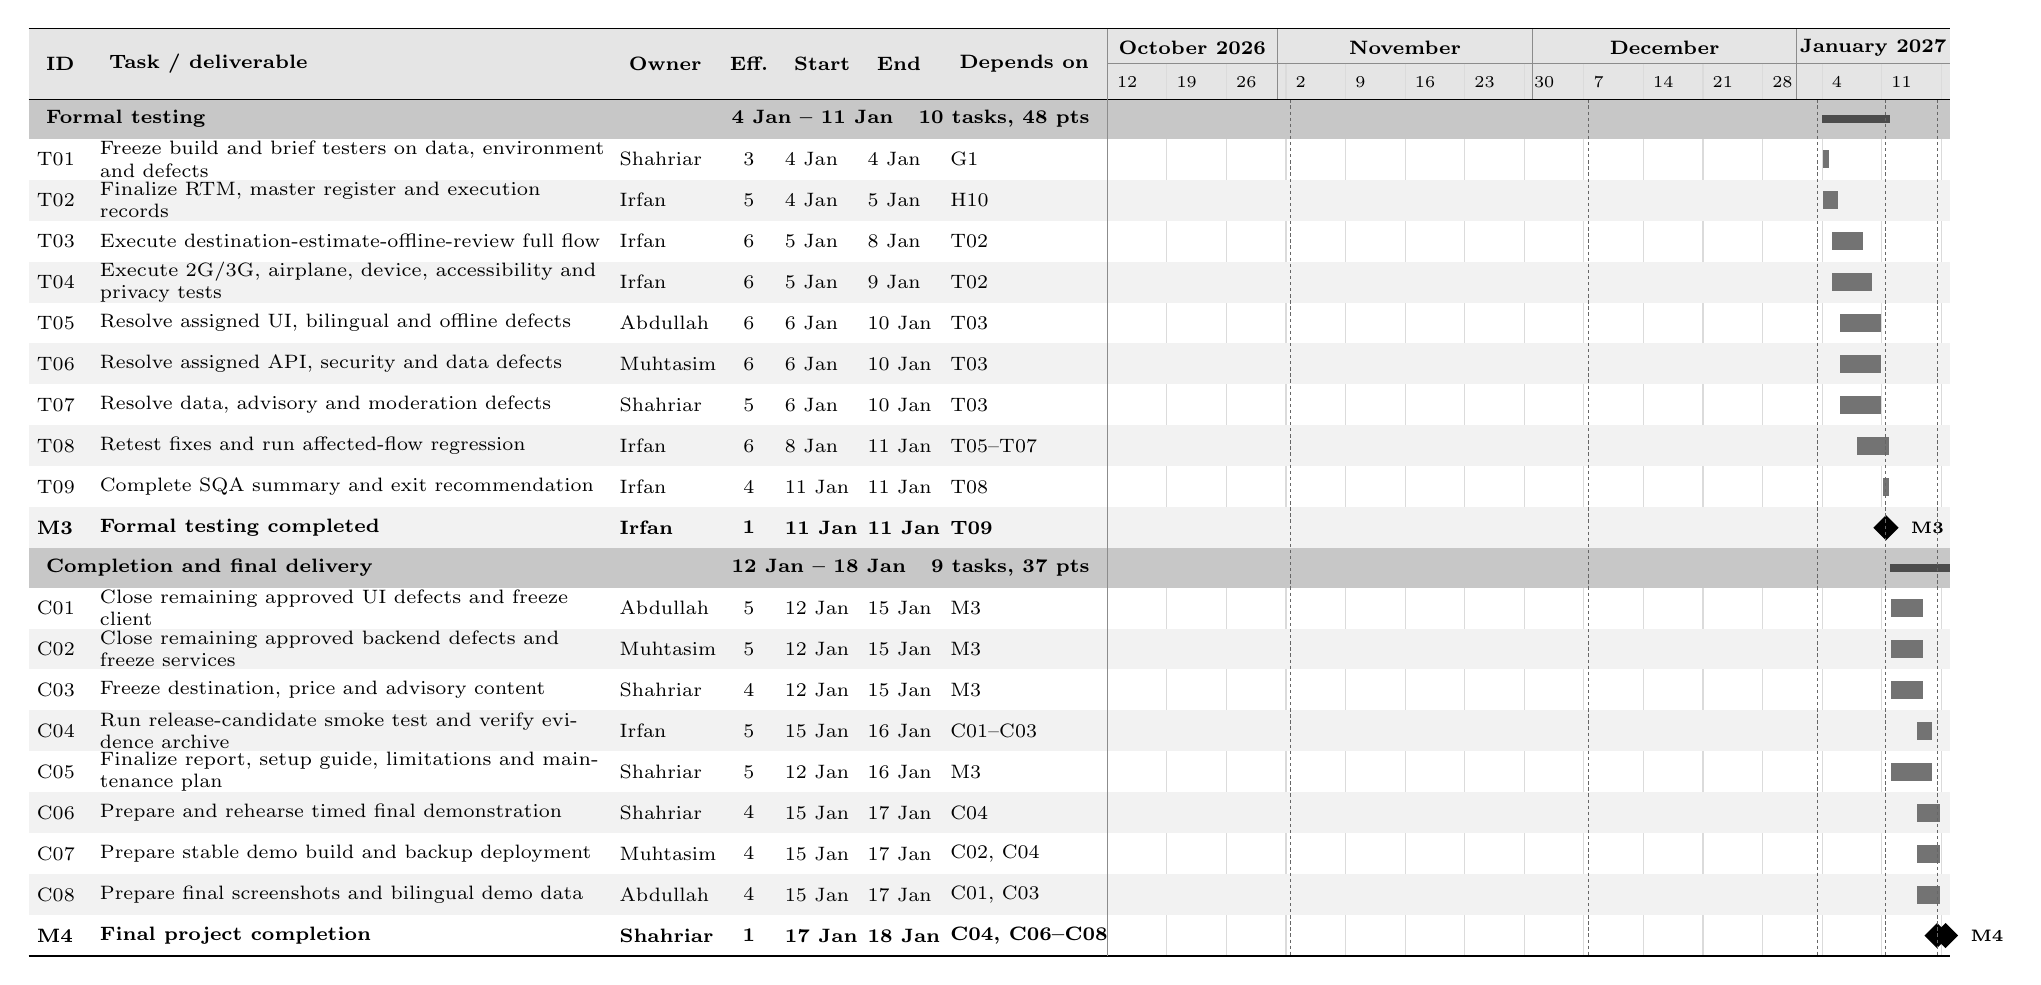
\begin{tikzpicture}[x=1mm,y=-1mm,font=\ganttfont]
\fill[black!10] (0,0) rectangle (244.0,9.0);
\node[anchor=west,font=\ganttfont\bfseries] at (1,4.5) {ID};
\node[anchor=west,font=\ganttfont\bfseries] at (9,4.5) {Task / deliverable};
\node[anchor=west,font=\ganttfont\bfseries] at (75,4.5) {Owner};
\node[anchor=center,font=\ganttfont\bfseries] at (91.5,4.5) {Eff.};
\node[anchor=west,font=\ganttfont\bfseries] at (96,4.5) {Start};
\node[anchor=west,font=\ganttfont\bfseries] at (106.5,4.5) {End};
\node[anchor=west,font=\ganttfont\bfseries] at (117,4.5) {Depends on};
\node[font=\ganttfont\bfseries] at (147.8080808080808,2.43) {October 2026};
\node[font=\ganttfont\bfseries] at (174.82828282828282,2.43) {November};
\draw[black!45] (158.6161616161616,0) -- (158.6161616161616,9.0);
\node[font=\ganttfont\bfseries] at (207.7929292929293,2.43) {December};
\draw[black!45] (191.04040404040404,0) -- (191.04040404040404,9.0);
\node[font=\ganttfont\bfseries] at (234.27272727272728,2.43) {January 2027};
\draw[black!45] (224.54545454545456,0) -- (224.54545454545456,9.0);
\draw[black!45] (137.0,4.5) -- (244.0,4.5);
\node[anchor=west,font=\ganttsmall] at (137.0,6.75) {12};
\node[anchor=west,font=\ganttsmall] at (144.56565656565655,6.75) {19};
\node[anchor=west,font=\ganttsmall] at (152.13131313131314,6.75) {26};
\node[anchor=west,font=\ganttsmall] at (159.6969696969697,6.75) {2};
\node[anchor=west,font=\ganttsmall] at (167.26262626262627,6.75) {9};
\node[anchor=west,font=\ganttsmall] at (174.82828282828282,6.75) {16};
\node[anchor=west,font=\ganttsmall] at (182.3939393939394,6.75) {23};
\node[anchor=west,font=\ganttsmall] at (189.95959595959596,6.75) {30};
\node[anchor=west,font=\ganttsmall] at (197.52525252525254,6.75) {7};
\node[anchor=west,font=\ganttsmall] at (205.0909090909091,6.75) {14};
\node[anchor=west,font=\ganttsmall] at (212.65656565656565,6.75) {21};
\node[anchor=west,font=\ganttsmall] at (220.22222222222223,6.75) {28};
\node[anchor=west,font=\ganttsmall] at (227.7878787878788,6.75) {4};
\node[anchor=west,font=\ganttsmall] at (235.35353535353536,6.75) {11};
\draw[black!14] (144.56565656565655,4.5) -- (144.56565656565655,117.80000000000004);
\draw[black!14] (152.13131313131314,4.5) -- (152.13131313131314,117.80000000000004);
\draw[black!14] (159.6969696969697,4.5) -- (159.6969696969697,117.80000000000004);
\draw[black!14] (167.26262626262627,4.5) -- (167.26262626262627,117.80000000000004);
\draw[black!14] (174.82828282828282,4.5) -- (174.82828282828282,117.80000000000004);
\draw[black!14] (182.3939393939394,4.5) -- (182.3939393939394,117.80000000000004);
\draw[black!14] (189.95959595959596,4.5) -- (189.95959595959596,117.80000000000004);
\draw[black!14] (197.52525252525254,4.5) -- (197.52525252525254,117.80000000000004);
\draw[black!14] (205.0909090909091,4.5) -- (205.0909090909091,117.80000000000004);
\draw[black!14] (212.65656565656565,4.5) -- (212.65656565656565,117.80000000000004);
\draw[black!14] (220.22222222222223,4.5) -- (220.22222222222223,117.80000000000004);
\draw[black!14] (227.7878787878788,4.5) -- (227.7878787878788,117.80000000000004);
\draw[black!14] (235.35353535353536,4.5) -- (235.35353535353536,117.80000000000004);
\draw[black!14] (242.91919191919192,4.5) -- (242.91919191919192,117.80000000000004);
\fill[black!22] (0,9.0) rectangle (244.0,14.0);
\node[anchor=west,font=\ganttfont\bfseries] at (1,11.5) {Formal testing};
\node[anchor=east,font=\ganttfont\bfseries] at (136.0,11.5) {4 Jan -- 11 Jan\quad 10 tasks, 48 pts};
\fill[black!70] (227.7878787878788,11.0) rectangle (236.43434343434345,12.0);
\node[anchor=west,inner sep=0pt,font=\ganttfont] at (1,16.6) {T01};
\node[anchor=west,text width=64mm,align=left,inner sep=0pt,font=\ganttfont] at (9,16.6) {Freeze build and brief testers on data, environment and defects};
\node[anchor=west,inner sep=0pt,font=\ganttfont] at (75,16.6) {Shahriar};
\node[anchor=center,inner sep=0pt,font=\ganttfont] at (91.5,16.6) {3};
\node[anchor=west,inner sep=0pt,font=\ganttfont] at (96,16.6) {4 Jan};
\node[anchor=west,inner sep=0pt,font=\ganttfont] at (106.5,16.6) {4 Jan};
\node[anchor=west,inner sep=0pt,font=\ganttfont] at (117,16.6) {G1};
\fill[black!55] (227.93787878787882,15.450000000000001) rectangle (228.7186868686869,17.75);
\fill[black!5] (0,19.2) rectangle (244.0,24.4);
\node[anchor=west,inner sep=0pt,font=\ganttfont] at (1,21.8) {T02};
\node[anchor=west,text width=64mm,align=left,inner sep=0pt,font=\ganttfont] at (9,21.8) {Finalize RTM, master register and execution records};
\node[anchor=west,inner sep=0pt,font=\ganttfont] at (75,21.8) {Irfan};
\node[anchor=center,inner sep=0pt,font=\ganttfont] at (91.5,21.8) {5};
\node[anchor=west,inner sep=0pt,font=\ganttfont] at (96,21.8) {4 Jan};
\node[anchor=west,inner sep=0pt,font=\ganttfont] at (106.5,21.8) {5 Jan};
\node[anchor=west,inner sep=0pt,font=\ganttfont] at (117,21.8) {H10};
\fill[black!55] (227.93787878787882,20.650000000000002) rectangle (229.79949494949497,22.95);
\node[anchor=west,inner sep=0pt,font=\ganttfont] at (1,27.0) {T03};
\node[anchor=west,text width=64mm,align=left,inner sep=0pt,font=\ganttfont] at (9,27.0) {Execute destination-estimate-offline-review full flow};
\node[anchor=west,inner sep=0pt,font=\ganttfont] at (75,27.0) {Irfan};
\node[anchor=center,inner sep=0pt,font=\ganttfont] at (91.5,27.0) {6};
\node[anchor=west,inner sep=0pt,font=\ganttfont] at (96,27.0) {5 Jan};
\node[anchor=west,inner sep=0pt,font=\ganttfont] at (106.5,27.0) {8 Jan};
\node[anchor=west,inner sep=0pt,font=\ganttfont] at (117,27.0) {T02};
\fill[black!55] (229.0186868686869,25.85) rectangle (233.0419191919192,28.15);
\fill[black!5] (0,29.599999999999998) rectangle (244.0,34.8);
\node[anchor=west,inner sep=0pt,font=\ganttfont] at (1,32.199999999999996) {T04};
\node[anchor=west,text width=64mm,align=left,inner sep=0pt,font=\ganttfont] at (9,32.199999999999996) {Execute 2G/3G, airplane, device, accessibility and privacy tests};
\node[anchor=west,inner sep=0pt,font=\ganttfont] at (75,32.199999999999996) {Irfan};
\node[anchor=center,inner sep=0pt,font=\ganttfont] at (91.5,32.199999999999996) {6};
\node[anchor=west,inner sep=0pt,font=\ganttfont] at (96,32.199999999999996) {5 Jan};
\node[anchor=west,inner sep=0pt,font=\ganttfont] at (106.5,32.199999999999996) {9 Jan};
\node[anchor=west,inner sep=0pt,font=\ganttfont] at (117,32.199999999999996) {T02};
\fill[black!55] (229.0186868686869,31.049999999999997) rectangle (234.12272727272727,33.349999999999994);
\node[anchor=west,inner sep=0pt,font=\ganttfont] at (1,37.4) {T05};
\node[anchor=west,text width=64mm,align=left,inner sep=0pt,font=\ganttfont] at (9,37.4) {Resolve assigned UI, bilingual and offline defects};
\node[anchor=west,inner sep=0pt,font=\ganttfont] at (75,37.4) {Abdullah};
\node[anchor=center,inner sep=0pt,font=\ganttfont] at (91.5,37.4) {6};
\node[anchor=west,inner sep=0pt,font=\ganttfont] at (96,37.4) {6 Jan};
\node[anchor=west,inner sep=0pt,font=\ganttfont] at (106.5,37.4) {10 Jan};
\node[anchor=west,inner sep=0pt,font=\ganttfont] at (117,37.4) {T03};
\fill[black!55] (230.09949494949498,36.25) rectangle (235.20353535353536,38.55);
\fill[black!5] (0,40.0) rectangle (244.0,45.2);
\node[anchor=west,inner sep=0pt,font=\ganttfont] at (1,42.6) {T06};
\node[anchor=west,text width=64mm,align=left,inner sep=0pt,font=\ganttfont] at (9,42.6) {Resolve assigned API, security and data defects};
\node[anchor=west,inner sep=0pt,font=\ganttfont] at (75,42.6) {Muhtasim};
\node[anchor=center,inner sep=0pt,font=\ganttfont] at (91.5,42.6) {6};
\node[anchor=west,inner sep=0pt,font=\ganttfont] at (96,42.6) {6 Jan};
\node[anchor=west,inner sep=0pt,font=\ganttfont] at (106.5,42.6) {10 Jan};
\node[anchor=west,inner sep=0pt,font=\ganttfont] at (117,42.6) {T03};
\fill[black!55] (230.09949494949498,41.45) rectangle (235.20353535353536,43.75);
\node[anchor=west,inner sep=0pt,font=\ganttfont] at (1,47.800000000000004) {T07};
\node[anchor=west,text width=64mm,align=left,inner sep=0pt,font=\ganttfont] at (9,47.800000000000004) {Resolve data, advisory and moderation defects};
\node[anchor=west,inner sep=0pt,font=\ganttfont] at (75,47.800000000000004) {Shahriar};
\node[anchor=center,inner sep=0pt,font=\ganttfont] at (91.5,47.800000000000004) {5};
\node[anchor=west,inner sep=0pt,font=\ganttfont] at (96,47.800000000000004) {6 Jan};
\node[anchor=west,inner sep=0pt,font=\ganttfont] at (106.5,47.800000000000004) {10 Jan};
\node[anchor=west,inner sep=0pt,font=\ganttfont] at (117,47.800000000000004) {T03};
\fill[black!55] (230.09949494949498,46.650000000000006) rectangle (235.20353535353536,48.95);
\fill[black!5] (0,50.400000000000006) rectangle (244.0,55.60000000000001);
\node[anchor=west,inner sep=0pt,font=\ganttfont] at (1,53.00000000000001) {T08};
\node[anchor=west,text width=64mm,align=left,inner sep=0pt,font=\ganttfont] at (9,53.00000000000001) {Retest fixes and run affected-flow regression};
\node[anchor=west,inner sep=0pt,font=\ganttfont] at (75,53.00000000000001) {Irfan};
\node[anchor=center,inner sep=0pt,font=\ganttfont] at (91.5,53.00000000000001) {6};
\node[anchor=west,inner sep=0pt,font=\ganttfont] at (96,53.00000000000001) {8 Jan};
\node[anchor=west,inner sep=0pt,font=\ganttfont] at (106.5,53.00000000000001) {11 Jan};
\node[anchor=west,inner sep=0pt,font=\ganttfont] at (117,53.00000000000001) {T05--T07};
\fill[black!55] (232.26111111111112,51.85000000000001) rectangle (236.28434343434344,54.150000000000006);
\node[anchor=west,inner sep=0pt,font=\ganttfont] at (1,58.20000000000001) {T09};
\node[anchor=west,text width=64mm,align=left,inner sep=0pt,font=\ganttfont] at (9,58.20000000000001) {Complete SQA summary and exit recommendation};
\node[anchor=west,inner sep=0pt,font=\ganttfont] at (75,58.20000000000001) {Irfan};
\node[anchor=center,inner sep=0pt,font=\ganttfont] at (91.5,58.20000000000001) {4};
\node[anchor=west,inner sep=0pt,font=\ganttfont] at (96,58.20000000000001) {11 Jan};
\node[anchor=west,inner sep=0pt,font=\ganttfont] at (106.5,58.20000000000001) {11 Jan};
\node[anchor=west,inner sep=0pt,font=\ganttfont] at (117,58.20000000000001) {T08};
\fill[black!55] (235.50353535353537,57.05000000000001) rectangle (236.28434343434344,59.35000000000001);
\fill[black!5] (0,60.80000000000001) rectangle (244.0,66.00000000000001);
\node[anchor=west,inner sep=0pt,font=\ganttfont\bfseries] at (1,63.40000000000001) {M3};
\node[anchor=west,text width=64mm,align=left,inner sep=0pt,font=\ganttfont\bfseries] at (9,63.40000000000001) {Formal testing completed};
\node[anchor=west,inner sep=0pt,font=\ganttfont\bfseries] at (75,63.40000000000001) {Irfan};
\node[anchor=center,inner sep=0pt,font=\ganttfont\bfseries] at (91.5,63.40000000000001) {1};
\node[anchor=west,inner sep=0pt,font=\ganttfont\bfseries] at (96,63.40000000000001) {11 Jan};
\node[anchor=west,inner sep=0pt,font=\ganttfont\bfseries] at (106.5,63.40000000000001) {11 Jan};
\node[anchor=west,inner sep=0pt,font=\ganttfont\bfseries] at (117,63.40000000000001) {T09};
\fill[black] (235.8939393939394,61.80000000000001) -- (237.4939393939394,63.40000000000001) -- (235.8939393939394,65.00000000000001) -- (234.2939393939394,63.40000000000001) -- cycle;
\node[anchor=west,font=\ganttsmall\bfseries] at (237.83434343434345,63.40000000000001) {M3};
\fill[black!22] (0,66.00000000000001) rectangle (244.0,71.00000000000001);
\node[anchor=west,font=\ganttfont\bfseries] at (1,68.50000000000001) {Completion and final delivery};
\node[anchor=east,font=\ganttfont\bfseries] at (136.0,68.50000000000001) {12 Jan -- 18 Jan\quad 9 tasks, 37 pts};
\fill[black!70] (236.43434343434345,68.00000000000001) rectangle (244.0,69.00000000000001);
\node[anchor=west,inner sep=0pt,font=\ganttfont] at (1,73.60000000000001) {C01};
\node[anchor=west,text width=64mm,align=left,inner sep=0pt,font=\ganttfont] at (9,73.60000000000001) {Close remaining approved UI defects and freeze client};
\node[anchor=west,inner sep=0pt,font=\ganttfont] at (75,73.60000000000001) {Abdullah};
\node[anchor=center,inner sep=0pt,font=\ganttfont] at (91.5,73.60000000000001) {5};
\node[anchor=west,inner sep=0pt,font=\ganttfont] at (96,73.60000000000001) {12 Jan};
\node[anchor=west,inner sep=0pt,font=\ganttfont] at (106.5,73.60000000000001) {15 Jan};
\node[anchor=west,inner sep=0pt,font=\ganttfont] at (117,73.60000000000001) {M3};
\fill[black!55] (236.58434343434345,72.45) rectangle (240.60757575757575,74.75000000000001);
\fill[black!5] (0,76.20000000000002) rectangle (244.0,81.40000000000002);
\node[anchor=west,inner sep=0pt,font=\ganttfont] at (1,78.80000000000001) {C02};
\node[anchor=west,text width=64mm,align=left,inner sep=0pt,font=\ganttfont] at (9,78.80000000000001) {Close remaining approved backend defects and freeze services};
\node[anchor=west,inner sep=0pt,font=\ganttfont] at (75,78.80000000000001) {Muhtasim};
\node[anchor=center,inner sep=0pt,font=\ganttfont] at (91.5,78.80000000000001) {5};
\node[anchor=west,inner sep=0pt,font=\ganttfont] at (96,78.80000000000001) {12 Jan};
\node[anchor=west,inner sep=0pt,font=\ganttfont] at (106.5,78.80000000000001) {15 Jan};
\node[anchor=west,inner sep=0pt,font=\ganttfont] at (117,78.80000000000001) {M3};
\fill[black!55] (236.58434343434345,77.65) rectangle (240.60757575757575,79.95000000000002);
\node[anchor=west,inner sep=0pt,font=\ganttfont] at (1,84.00000000000001) {C03};
\node[anchor=west,text width=64mm,align=left,inner sep=0pt,font=\ganttfont] at (9,84.00000000000001) {Freeze destination, price and advisory content};
\node[anchor=west,inner sep=0pt,font=\ganttfont] at (75,84.00000000000001) {Shahriar};
\node[anchor=center,inner sep=0pt,font=\ganttfont] at (91.5,84.00000000000001) {4};
\node[anchor=west,inner sep=0pt,font=\ganttfont] at (96,84.00000000000001) {12 Jan};
\node[anchor=west,inner sep=0pt,font=\ganttfont] at (106.5,84.00000000000001) {15 Jan};
\node[anchor=west,inner sep=0pt,font=\ganttfont] at (117,84.00000000000001) {M3};
\fill[black!55] (236.58434343434345,82.85000000000001) rectangle (240.60757575757575,85.15000000000002);
\fill[black!5] (0,86.60000000000002) rectangle (244.0,91.80000000000003);
\node[anchor=west,inner sep=0pt,font=\ganttfont] at (1,89.20000000000002) {C04};
\node[anchor=west,text width=64mm,align=left,inner sep=0pt,font=\ganttfont] at (9,89.20000000000002) {Run release-candidate smoke test and verify evidence archive};
\node[anchor=west,inner sep=0pt,font=\ganttfont] at (75,89.20000000000002) {Irfan};
\node[anchor=center,inner sep=0pt,font=\ganttfont] at (91.5,89.20000000000002) {5};
\node[anchor=west,inner sep=0pt,font=\ganttfont] at (96,89.20000000000002) {15 Jan};
\node[anchor=west,inner sep=0pt,font=\ganttfont] at (106.5,89.20000000000002) {16 Jan};
\node[anchor=west,inner sep=0pt,font=\ganttfont] at (117,89.20000000000002) {C01--C03};
\fill[black!55] (239.82676767676767,88.05000000000001) rectangle (241.68838383838383,90.35000000000002);
\node[anchor=west,inner sep=0pt,font=\ganttfont] at (1,94.40000000000002) {C05};
\node[anchor=west,text width=64mm,align=left,inner sep=0pt,font=\ganttfont] at (9,94.40000000000002) {Finalize report, setup guide, limitations and maintenance plan};
\node[anchor=west,inner sep=0pt,font=\ganttfont] at (75,94.40000000000002) {Shahriar};
\node[anchor=center,inner sep=0pt,font=\ganttfont] at (91.5,94.40000000000002) {5};
\node[anchor=west,inner sep=0pt,font=\ganttfont] at (96,94.40000000000002) {12 Jan};
\node[anchor=west,inner sep=0pt,font=\ganttfont] at (106.5,94.40000000000002) {16 Jan};
\node[anchor=west,inner sep=0pt,font=\ganttfont] at (117,94.40000000000002) {M3};
\fill[black!55] (236.58434343434345,93.25000000000001) rectangle (241.68838383838383,95.55000000000003);
\fill[black!5] (0,97.00000000000003) rectangle (244.0,102.20000000000003);
\node[anchor=west,inner sep=0pt,font=\ganttfont] at (1,99.60000000000002) {C06};
\node[anchor=west,text width=64mm,align=left,inner sep=0pt,font=\ganttfont] at (9,99.60000000000002) {Prepare and rehearse timed final demonstration};
\node[anchor=west,inner sep=0pt,font=\ganttfont] at (75,99.60000000000002) {Shahriar};
\node[anchor=center,inner sep=0pt,font=\ganttfont] at (91.5,99.60000000000002) {4};
\node[anchor=west,inner sep=0pt,font=\ganttfont] at (96,99.60000000000002) {15 Jan};
\node[anchor=west,inner sep=0pt,font=\ganttfont] at (106.5,99.60000000000002) {17 Jan};
\node[anchor=west,inner sep=0pt,font=\ganttfont] at (117,99.60000000000002) {C04};
\fill[black!55] (239.82676767676767,98.45000000000002) rectangle (242.7691919191919,100.75000000000003);
\node[anchor=west,inner sep=0pt,font=\ganttfont] at (1,104.80000000000003) {C07};
\node[anchor=west,text width=64mm,align=left,inner sep=0pt,font=\ganttfont] at (9,104.80000000000003) {Prepare stable demo build and backup deployment};
\node[anchor=west,inner sep=0pt,font=\ganttfont] at (75,104.80000000000003) {Muhtasim};
\node[anchor=center,inner sep=0pt,font=\ganttfont] at (91.5,104.80000000000003) {4};
\node[anchor=west,inner sep=0pt,font=\ganttfont] at (96,104.80000000000003) {15 Jan};
\node[anchor=west,inner sep=0pt,font=\ganttfont] at (106.5,104.80000000000003) {17 Jan};
\node[anchor=west,inner sep=0pt,font=\ganttfont] at (117,104.80000000000003) {C02, C04};
\fill[black!55] (239.82676767676767,103.65000000000002) rectangle (242.7691919191919,105.95000000000003);
\fill[black!5] (0,107.40000000000003) rectangle (244.0,112.60000000000004);
\node[anchor=west,inner sep=0pt,font=\ganttfont] at (1,110.00000000000003) {C08};
\node[anchor=west,text width=64mm,align=left,inner sep=0pt,font=\ganttfont] at (9,110.00000000000003) {Prepare final screenshots and bilingual demo data};
\node[anchor=west,inner sep=0pt,font=\ganttfont] at (75,110.00000000000003) {Abdullah};
\node[anchor=center,inner sep=0pt,font=\ganttfont] at (91.5,110.00000000000003) {4};
\node[anchor=west,inner sep=0pt,font=\ganttfont] at (96,110.00000000000003) {15 Jan};
\node[anchor=west,inner sep=0pt,font=\ganttfont] at (106.5,110.00000000000003) {17 Jan};
\node[anchor=west,inner sep=0pt,font=\ganttfont] at (117,110.00000000000003) {C01, C03};
\fill[black!55] (239.82676767676767,108.85000000000002) rectangle (242.7691919191919,111.15000000000003);
\node[anchor=west,inner sep=0pt,font=\ganttfont\bfseries] at (1,115.20000000000003) {M4};
\node[anchor=west,text width=64mm,align=left,inner sep=0pt,font=\ganttfont\bfseries] at (9,115.20000000000003) {Final project completion};
\node[anchor=west,inner sep=0pt,font=\ganttfont\bfseries] at (75,115.20000000000003) {Shahriar};
\node[anchor=center,inner sep=0pt,font=\ganttfont\bfseries] at (91.5,115.20000000000003) {1};
\node[anchor=west,inner sep=0pt,font=\ganttfont\bfseries] at (96,115.20000000000003) {17 Jan};
\node[anchor=west,inner sep=0pt,font=\ganttfont\bfseries] at (106.5,115.20000000000003) {18 Jan};
\node[anchor=west,inner sep=0pt,font=\ganttfont\bfseries] at (117,115.20000000000003) {C04, C06--C08};
\fill[black] (242.37878787878788,113.60000000000004) -- (243.97878787878787,115.20000000000003) -- (242.37878787878788,116.80000000000003) -- (240.77878787878788,115.20000000000003) -- cycle;
\fill[black] (243.45959595959596,113.60000000000004) -- (245.05959595959595,115.20000000000003) -- (243.45959595959596,116.80000000000003) -- (241.85959595959596,115.20000000000003) -- cycle;
\node[anchor=west,font=\ganttsmall\bfseries] at (245.4,115.20000000000003) {M4};
\draw[black!60,dash pattern=on 1.2pt off 1pt,line width=0.35pt] (160.23737373737373,9.0) -- (160.23737373737373,117.80000000000004);
\draw[black!60,dash pattern=on 1.2pt off 1pt,line width=0.35pt] (198.06565656565658,9.0) -- (198.06565656565658,117.80000000000004);
\draw[black!60,dash pattern=on 1.2pt off 1pt,line width=0.35pt] (227.24747474747477,9.0) -- (227.24747474747477,117.80000000000004);
\draw[black!60,dash pattern=on 1.2pt off 1pt,line width=0.35pt] (235.8939393939394,9.0) -- (235.8939393939394,117.80000000000004);
\draw[black!60,dash pattern=on 1.2pt off 1pt,line width=0.35pt] (242.37878787878788,9.0) -- (242.37878787878788,117.80000000000004);
\draw[line width=0.6pt] (0,0) -- (244.0,0);
\draw[line width=0.4pt] (0,9.0) -- (244.0,9.0);
\draw[line width=0.6pt] (0,117.80000000000004) -- (244.0,117.80000000000004);
\draw[black!45] (137.0,0) -- (137.0,117.80000000000004);
\end{tikzpicture}
}
\end{minipage}
\end{landscape}}

% =====================================================================
\section{Risk Assessment}
{\small
\begin{longtable}{L{30mm}C{13mm}L{39mm}L{59mm}}
\caption{Risk register with early warnings and mitigation}\label{tab:risks}\\
\toprule
\hd{Risk} & \hd{Level} & \hd{Early warning} & \hd{Mitigation and owner} \\
\midrule
\endfirsthead
\multicolumn{4}{l}{\small\textbf{Table \thetable} (continued)}\\
\toprule
\hd{Risk} & \hd{Level} & \hd{Early warning} & \hd{Mitigation and owner} \\
\midrule
\endhead
\bottomrule
\endlastfoot
Scope growth & High & New features requested during a cycle & Freeze the semester capabilities. Any addition replaces work of equal effort. Owner: Shahriar. \\
Insufficient destination or price data & High & Missing sources or conflicting values & Begin research in the first cycle. Store provenance, date, unit, tier, and confidence. Owners: all content owners. \\
Weak estimator accuracy & High & Large error on development cases & Use ranges, transparent rules, a baseline, and sealed held-out trips. Owners: Shahriar and Irfan. \\
Stale safety information & High & Advisory lacks a current official source & Store verification and validity dates. Recheck before publication and demonstrations. Owners: destination owners. \\
Offline storage eviction & Medium & Persistence is refused or a pack disappears & Show status, re-download, and delete controls. Test on real devices. Owners: Abdullah and Irfan. \\
Authentication delay & Medium & Account API misses the planned cycle & Continue the guest destination and pack slice. Complete accounts early in the next cycle. Owner: Muhtasim. \\
Team unavailability & High & Missed review or unmerged work & Maintain shared documentation, small reviewed changes, tests, and a backup owner for each module. Owner: Shahriar. \\
Privacy or security defect & High & Sensitive data appears in logs, cache, or pack & Apply data minimisation, network-only private APIs, security tests, and a release gate. Owners: Muhtasim and Irfan. \\
Bangla rendering failure & Medium & Broken conjuncts or unreadable wrapping & Use system-font fallback and a device-version test matrix. Owner: Abdullah. \\
Low pilot participation & Medium & Fewer than eight usable participants & Recruit early and maintain backup participants. Owner: Irfan. \\
Copyright issue & Medium & Image or source has unclear permission & Use owned or openly licensed images and record licences. Owner: each content owner. \\
Deadline pressure & High & The 7 December target or testing entry is at risk & Review scope at the checkpoint and protect the fixed testing and final dates. Owners: Shahriar and team. \\
\end{longtable}
}

% =====================================================================
\section{Feasibility Study}
\subsection{Technical Feasibility}
The selected technologies match the team roles. React and TypeScript support the bilingual frontend. FastAPI supports the API layer. PostgreSQL provides authoritative relational storage. Workbox manages the versioned application shell. IndexedDB through Dexie stores downloaded packs, saved trip briefs, and review drafts. Authenticated API responses are excluded from public service-worker caches.

The MVP avoids dependencies on real payments, SMS gateways, NID verification, live inventory, and native application packaging. The highest-risk capability, offline access, is tested with one complete destination before the first milestone. The architecture is therefore achievable by the team within the semester.

\subsection{Economic and Financial Feasibility}
The MVP uses open-source frameworks and existing student hardware. The figures below are planning allowances, not quotations.

\begin{table}[!htbp]
\centering
\caption{Semester cost allowance}\label{tab:budget}
{\small
\begin{tabularx}{\textwidth}{Y R{26mm} L{62mm}}
\toprule
\hd{Cost category} & \hd{Estimated BDT} & \hd{Basis} \\
\midrule
Development frameworks and database & 0 & Open-source software \\
Existing laptops and Android test phones & 0 & Team-owned equipment \\
Test connectivity, calls, and data collection & 1,500 & Pilot and source-verification allowance \\
Optional domain and short-term hosting & 2,500 & Used only if an external demonstration requires it \\
Contingency & 2,000 & Unexpected testing or deployment expense \\
\midrule
\textbf{Planning ceiling} & \textbf{6,000} & Maximum proposed semester allowance \\
\bottomrule
\end{tabularx}
}
\end{table}

The future business model can include vendor subscriptions, booking commissions, clearly labelled sponsorship, and optional premium services. Sponsorship must not affect ratings or moderation.

\subsection{Schedule and Time Feasibility}
The Gantt chart assigns dependencies, evidence, risk notes, and effort to each task, and workload is balanced at 87 primary effort points per member. The first complete vertical slice is due on 2 November. The 7 December checkpoint leaves time to reduce destination quantity before reducing quality. Formal testing has a protected eight-day window, followed by a final correction and release period.

If work falls behind, the team will remove future-phase functions before changing core acceptance criteria. Real booking, real payment, group tours, and advanced verification remain outside the semester dependency chain.

\subsection{Operational and Ethical Feasibility}
Pilot participation is voluntary and uses a short consent notice. The project does not collect real NID records, payment credentials, or unnecessary personal documents. Optional contacts remain local to the user's device. Abhijatri will not present itself as an emergency-response or traveller-monitoring service. Restrictions and advisories must be verified again before publication or demonstration.

\subsection{Feasibility Conclusion}
Abhijatri is feasible as a semester project if the team preserves the MVP boundary and treats commercial and social expansion as future work. The selected technology is available, direct academic cost is limited, risk is tested early, and the schedule includes formal acceptance evidence.

\end{document}
